% Options for packages loaded elsewhere
\PassOptionsToPackage{unicode}{hyperref}
\PassOptionsToPackage{hyphens}{url}
\PassOptionsToPackage{dvipsnames,svgnames,x11names}{xcolor}
%
\documentclass[
  letterpaper,
  DIV=11,
  numbers=noendperiod]{scrartcl}

\usepackage{amsmath,amssymb}
\usepackage{iftex}
\ifPDFTeX
  \usepackage[T1]{fontenc}
  \usepackage[utf8]{inputenc}
  \usepackage{textcomp} % provide euro and other symbols
\else % if luatex or xetex
  \usepackage{unicode-math}
  \defaultfontfeatures{Scale=MatchLowercase}
  \defaultfontfeatures[\rmfamily]{Ligatures=TeX,Scale=1}
\fi
\usepackage{lmodern}
\ifPDFTeX\else  
    % xetex/luatex font selection
\fi
% Use upquote if available, for straight quotes in verbatim environments
\IfFileExists{upquote.sty}{\usepackage{upquote}}{}
\IfFileExists{microtype.sty}{% use microtype if available
  \usepackage[]{microtype}
  \UseMicrotypeSet[protrusion]{basicmath} % disable protrusion for tt fonts
}{}
\makeatletter
\@ifundefined{KOMAClassName}{% if non-KOMA class
  \IfFileExists{parskip.sty}{%
    \usepackage{parskip}
  }{% else
    \setlength{\parindent}{0pt}
    \setlength{\parskip}{6pt plus 2pt minus 1pt}}
}{% if KOMA class
  \KOMAoptions{parskip=half}}
\makeatother
\usepackage{xcolor}
\setlength{\emergencystretch}{3em} % prevent overfull lines
\setcounter{secnumdepth}{5}
% Make \paragraph and \subparagraph free-standing
\ifx\paragraph\undefined\else
  \let\oldparagraph\paragraph
  \renewcommand{\paragraph}[1]{\oldparagraph{#1}\mbox{}}
\fi
\ifx\subparagraph\undefined\else
  \let\oldsubparagraph\subparagraph
  \renewcommand{\subparagraph}[1]{\oldsubparagraph{#1}\mbox{}}
\fi


\providecommand{\tightlist}{%
  \setlength{\itemsep}{0pt}\setlength{\parskip}{0pt}}\usepackage{longtable,booktabs,array}
\usepackage{calc} % for calculating minipage widths
% Correct order of tables after \paragraph or \subparagraph
\usepackage{etoolbox}
\makeatletter
\patchcmd\longtable{\par}{\if@noskipsec\mbox{}\fi\par}{}{}
\makeatother
% Allow footnotes in longtable head/foot
\IfFileExists{footnotehyper.sty}{\usepackage{footnotehyper}}{\usepackage{footnote}}
\makesavenoteenv{longtable}
\usepackage{graphicx}
\makeatletter
\def\maxwidth{\ifdim\Gin@nat@width>\linewidth\linewidth\else\Gin@nat@width\fi}
\def\maxheight{\ifdim\Gin@nat@height>\textheight\textheight\else\Gin@nat@height\fi}
\makeatother
% Scale images if necessary, so that they will not overflow the page
% margins by default, and it is still possible to overwrite the defaults
% using explicit options in \includegraphics[width, height, ...]{}
\setkeys{Gin}{width=\maxwidth,height=\maxheight,keepaspectratio}
% Set default figure placement to htbp
\makeatletter
\def\fps@figure{htbp}
\makeatother
% definitions for citeproc citations
\NewDocumentCommand\citeproctext{}{}
\NewDocumentCommand\citeproc{mm}{%
  \begingroup\def\citeproctext{#2}\cite{#1}\endgroup}
\makeatletter
 % allow citations to break across lines
 \let\@cite@ofmt\@firstofone
 % avoid brackets around text for \cite:
 \def\@biblabel#1{}
 \def\@cite#1#2{{#1\if@tempswa , #2\fi}}
\makeatother
\newlength{\cslhangindent}
\setlength{\cslhangindent}{1.5em}
\newlength{\csllabelwidth}
\setlength{\csllabelwidth}{3em}
\newenvironment{CSLReferences}[2] % #1 hanging-indent, #2 entry-spacing
 {\begin{list}{}{%
  \setlength{\itemindent}{0pt}
  \setlength{\leftmargin}{0pt}
  \setlength{\parsep}{0pt}
  % turn on hanging indent if param 1 is 1
  \ifodd #1
   \setlength{\leftmargin}{\cslhangindent}
   \setlength{\itemindent}{-1\cslhangindent}
  \fi
  % set entry spacing
  \setlength{\itemsep}{#2\baselineskip}}}
 {\end{list}}
\usepackage{calc}
\newcommand{\CSLBlock}[1]{\hfill\break\parbox[t]{\linewidth}{\strut\ignorespaces#1\strut}}
\newcommand{\CSLLeftMargin}[1]{\parbox[t]{\csllabelwidth}{\strut#1\strut}}
\newcommand{\CSLRightInline}[1]{\parbox[t]{\linewidth - \csllabelwidth}{\strut#1\strut}}
\newcommand{\CSLIndent}[1]{\hspace{\cslhangindent}#1}

\usepackage{booktabs}
\usepackage{longtable}
\usepackage{array}
\usepackage{multirow}
\usepackage{wrapfig}
\usepackage{float}
\usepackage{colortbl}
\usepackage{pdflscape}
\usepackage{tabu}
\usepackage{threeparttable}
\usepackage{threeparttablex}
\usepackage[normalem]{ulem}
\usepackage{makecell}
\usepackage{xcolor}
\KOMAoption{captions}{tableheading}
\makeatletter
\@ifpackageloaded{caption}{}{\usepackage{caption}}
\AtBeginDocument{%
\ifdefined\contentsname
  \renewcommand*\contentsname{Table of contents}
\else
  \newcommand\contentsname{Table of contents}
\fi
\ifdefined\listfigurename
  \renewcommand*\listfigurename{List of Figures}
\else
  \newcommand\listfigurename{List of Figures}
\fi
\ifdefined\listtablename
  \renewcommand*\listtablename{List of Tables}
\else
  \newcommand\listtablename{List of Tables}
\fi
\ifdefined\figurename
  \renewcommand*\figurename{Figure}
\else
  \newcommand\figurename{Figure}
\fi
\ifdefined\tablename
  \renewcommand*\tablename{Table}
\else
  \newcommand\tablename{Table}
\fi
}
\@ifpackageloaded{float}{}{\usepackage{float}}
\floatstyle{ruled}
\@ifundefined{c@chapter}{\newfloat{codelisting}{h}{lop}}{\newfloat{codelisting}{h}{lop}[chapter]}
\floatname{codelisting}{Listing}
\newcommand*\listoflistings{\listof{codelisting}{List of Listings}}
\captionsetup{labelsep=colon}
\makeatother
\makeatletter
\makeatother
\makeatletter
\@ifpackageloaded{caption}{}{\usepackage{caption}}
\@ifpackageloaded{subcaption}{}{\usepackage{subcaption}}
\makeatother
\ifLuaTeX
  \usepackage{selnolig}  % disable illegal ligatures
\fi
\usepackage{bookmark}

\IfFileExists{xurl.sty}{\usepackage{xurl}}{} % add URL line breaks if available
\urlstyle{same} % disable monospaced font for URLs
\hypersetup{
  pdftitle={古今和歌集の現代語訳における追加率と追加要素の分析},
  pdfauthor={Xudong Chen; Bor Hodošček; Hilofumi Yamamoto},
  pdfkeywords={歌ことば, 現代語訳, ノンリテラル情報},
  colorlinks=true,
  linkcolor={blue},
  filecolor={Maroon},
  citecolor={Blue},
  urlcolor={Blue},
  pdfcreator={LaTeX via pandoc}}

\title{古今和歌集の現代語訳における追加率と追加要素の分析}
\author{Xudong Chen \and Bor Hodošček \and Hilofumi Yamamoto}
\date{2024-09-01}

\begin{document}
\maketitle
\begin{abstract}
筆者らは、古今和歌集の歌ことばのノンリテラル情報を可視化するシステムを開発してきたが、それに用いた現代語訳や追加要素の詳細な分析は行われていなかった。本研究の目的は、古今和歌集の現代語訳10種類が、ノンリテラル要素の可視化に適しているかどうかを分析することである。まず、現代語訳について概観し、訳者の翻訳意識を作意中心・テキスト中心・読者中心・不明の4種に分類した。次に、直訳語を持たない歌ことばの割合(不一致率)と、現代語訳における追加要素の割合(追加率)を計算し、どの訳も多くの追加要素を含むことを確認した。さらに、具体例を示し、コーパスレベルの共出現傾向に基づく推論が現代語訳にどのように反映されているかを分析した。これにより、現代語訳がノンリテラル情報の可視化に適用できることを示した。
Previous research has developed a system for visualizing non-literal
information in the Kokinshū's poetic words by adding elements in
translations found in annotated bookss. However, detailed analysis of
these translations and the added elements has not been conducted. This
study aims to evaluate whether the ten contemporary Japanese
translations of the Kokinshū used in prior studies are suitable for
visualizing non-literal elements. First, we review these translations
and categorize the translators' approaches as poet-focused,
text-focused, reader-focused, or unclear. We then calculate the unmatch
rate (the proportion of poetic words without direct equivalents) and the
addition rate (the proportion of added elements) to see how elements
were incorporated. Finally, we provide case analyses of specific
examples, showing how corpus-level co-occurrence tendencies influenced
the addition of elements to clarify meanings. Our findings show that
despite varied approaches, the translations contain similar levels of
added elements, suggesting that contemporary translations can
effectively visualize the non-literal aspects of the Kokinshū's original
text.
\end{abstract}

\renewcommand*\contentsname{目次}
{
\hypersetup{linkcolor=}
\setcounter{tocdepth}{3}
\tableofcontents
}
\section{はじめに}\label{ux306fux3058ux3081ux306b}

\subsection{目的と結論の概要}\label{ux76eeux7684ux3068ux7d50ux8ad6ux306eux6982ux8981}

本稿の目的は、和歌の現代語訳が、直訳や逐語訳であっても、訳者の意図が異なっても、ノンリテラル要素を補足する解釈材料として利用できるかを検討することである。この目的を達成するため、原文との不一致率と訳文における追加率を計算し、さらに具体的な事例を通じて追加要素の分析を行った。

具体的には、和歌の現代語訳におけるノンリテラル要素の可視化とその応用可能性について検討した。古今和歌集の口語訳の歴史的な変遷を俯瞰し、20世紀における注釈書10種類の現代語訳に見られる翻訳アプローチを分類した。また、古語と現代語訳の語レベルの不一致率と現代語訳における追加率を計算し、翻訳アプローチにかかわらず、現代語訳にノンリテラル要素が追加されていることと、原文要素の欠落が避けられている傾向を確認した。これにより、現代語訳が直訳や逐語訳にとどまらず、原文の理解を補足する役割を果たしている可能性が示された。さらに、具体的な現代語訳の事例を提示し、対象語のコーパスレベルの共出現語、共出現語の全体的な志向性がセンテンスレベルの現代語訳それぞれに反映されているかどうかを検討した。以上の結果から、現代語訳をノンリテラル情報の可視化への応用が現実的であることを示した。

\subsection{背景}\label{ux80ccux666f}

和歌に見られるノンリテラル要素の概要を説明し、現代語訳を用いたこれらの要素の可視化に関する問題や課題について述べる。これまでの研究において素材の分析が十分に行われていなかった点を指摘し、翻訳および関連研究の紹介を通して、その意義を再確認する。

\subsubsection{和歌と和歌におけるノンリテラル要素}\label{ux548cux6b4cux3068ux548cux6b4cux306bux304aux3051ux308bux30ceux30f3ux30eaux30c6ux30e9ux30ebux8981ux7d20}

古今和歌集仮名序に見られるように、歌人は「心に思ふもの」を自然界の物事に託して表現することが多く、直接的に明言することは稀である。和歌のことば(以下「歌ことば」)を字義通りに理解したとしても、その「心に思ふもの」には直接アクセスすることはできない。例えば、古今集の恋の歌を例にとると、

\begin{quote}
初雁の鳴きこそわたれ世の中の人の心の秋しうければ(古今・恋五・貫之)
\end{quote}

この歌を字義通りに解釈すれば、各語の意味は理解できるかもしれないが、「心に思ふもの」を読み取ることは難しい\footnote{初雁が鳴いて渡ってくるのだが、人の心の秋が来るのが悲しいので(筆者訳)}。しかし、歌ことば辞典で「秋【あき】」(片桐
1983, 3)
を調べると、リテラルな意味では意図的に表現しない、あるいは客観的に表現できない情報が含まれていることに気づく。

\begin{quote}
秋【あき】
{[}\ldots{]}「秋」と「飽」を掛け、過ぎ去ってゆく秋と過ぎ去ってゆく愛を惜しむことが多かった。【脚注】{[}雁の{]}「鳴く」を人が「泣く」と同列にしか把握しない
{[}\ldots{]}(片桐 1983, 3)
\end{quote}

片桐 (1983, 3)
によると、恋人の心が「飽き(秋)」て、歌人が「泣(鳴)」いている「失恋」の物語と解釈することができる。このように、「秋」という表現から読み取る「飽きる恋」の情報は、原文の文脈(周辺語)ではノンリテラルであり、語の字義通りの意味だけでは受け取れない。和歌の深い意味を引き出すためには、表面的な字義を超えたノンリテラルな解釈が求められることがわかる。

\subsubsection{現代語訳の追加要素に基づく歌ことばのノンリテラル要素の可視化}\label{ux73feux4ee3ux8a9eux8a33ux306eux8ffdux52a0ux8981ux7d20ux306bux57faux3065ux304fux6b4cux3053ux3068ux3070ux306eux30ceux30f3ux30eaux30c6ux30e9ux30ebux8981ux7d20ux306eux53efux8996ux5316}

筆者らはこれまで、古今和歌集の10種類の現代日本語訳を基に、歌ことばのノンリテラル要素を可視化するシステムを開発してきた
(Yamamoto 2005, 2006; Chen, Yamamoto, and Hodošček
2024)。このシステムは、古語と現代語訳を比較し、浮かび上がる補足要素によってノンリテラル情報を可視化している。この手法は、近藤みゆき.
(2001) と 近藤泰弘. (2011)
によって「引き算」とも呼ばれている。ただし、引き算で残る現代語訳の追加要素がどのような性質を持ち、ノンリテラル要素として扱えるかについては、より詳細な検討が必要である。
翻訳における要素の追加について、Koller ({[}2004{]} 1979, 249)
は、翻訳者の「介入
(Eingriff)」であり、原作を尊重し、価値を変えない形で、読者の不足する背景知識やデノテーション・コノテーション情報、言語内的、社会文化的、間テキスト的な情報
(intertextual information) を補うことが含まれると指摘している (Koller
{[}2004{]} 1979,
249)。これにより、翻訳は注釈や辞書と同様に、ノンリテラル情報を解釈するための有効な資料となる。
しかし、翻訳の追加要素は、読者の理解力を過大評価または過小評価した結果として現れる場合もある
(Nida 1964, 155; Koller {[}2004{]} 1979,
249--50)。そのため、訳者による翻訳の追加要素のバリエーションを無視することはできない。古今和歌集の歌ことばを解釈する資料として現代語訳が有用であると
Chen, Yamamoto, and Hodošček (2024)
でも言及されているが、そのバリエーションについては十分な説明が行われていない。和歌の口語訳の背景や訳者毎の翻訳アプローチを再検討する必要がある。
本稿では、これまで使用してきた10種類の現代語訳について、その成立背景や追加要素の量的および質的な分析を行う。翻訳における追加要素が読者の理解力を反映して生成されたものである可能性を考慮し、異なる訳者が和歌のノンリテラル要素をどの程度表現できたかを検討する。訳者の翻訳アプローチを整理し、その違いを明らかにすることで、翻訳の普遍的な課題と限界を考察する。
この分析により、ノンリテラル要素の可視化システムの根拠をより明確にし、その改善の方向性を示すことができる。次節では、材料について説明を行う。

\section{データ:古今集、注釈と現代語訳}\label{sec-materials}

本節では、材料として使用する古今集の概要を説明し、和歌、古今集、注釈書、そしてその現代語訳の歴史的背景について概観する。

\subsection{古今集}\label{ux53e4ux4ecaux96c6}

和歌は「歌」と称されるように、もともと宮廷で声を上げて詠まれるものであり、当時の話しことばが基礎となっている。古今集は、その名が示す通り、古代の歌と当時の歌を集めたものであり、『万葉集』に収められた7世紀から8世紀の和歌も含まれている。これには、山部赤人、柿本人麻呂、額田王など、和歌史において重要な歌人の作品が仮名で記録されている。

また、古今集は、後に続く勅撰和歌集(二十一代集)の先駆けとして成立し、和歌の基本的な形式を確立した。編者である紀貫之による「仮名序」は、和歌の理論書としても位置付けられており、後の和歌文学や日本文学全般において重要な資料となっている。「源氏物語」「土佐日記」「伊勢物語」などの古典作品に多くの和歌が引用されていることからも、古今集は文学研究の基本資料としての役割を果たしている。また、話しことばの特徴を持つことから、日本語の歴史的変遷を知る上でも貴重な資料である。

\subsection{古今集の注釈と現代日本語訳}\label{ux53e4ux4ecaux96c6ux306eux6ce8ux91c8ux3068ux73feux4ee3ux65e5ux672cux8a9eux8a33}

古今集は、日本古典文学の中で多くの注釈書を生み出しており、それ自体が一つの研究分野として確立されている
(窪田 1960,
上中下:319)。これらの注釈書に含まれる現代語訳は、主に読者が和歌を理解しやすくするために書かれており、翻訳家の目的は和歌の解釈を伝えることにある。ここでは、近代以前と近代以降の注釈の歴史を簡単に概観し、特に明治以降に注釈書に掲載された現代語訳について考察する。

近代(1868年)以前には、多くの古今集の注釈書が出版されており、1600年から1868年の間に70以上の注釈書が存在している
(小島 and 新井 1989, 447--50)。表 Table~\ref{tbl-annotation}
に、近代以前の代表的な注釈書を5つ示す。

北村季吟の『八代集抄』は、古今集を含む8つの勅撰和歌集\footnote{八代集とは、古今集、後撰集、拾遺集、後拾遺集、金葉集、詞花集、千載集、新古今集の8つの勅撰和歌集を指す。}を対象とした注釈書であり、108巻(50冊)にも及ぶ大著である。契沖(1640--1701)の『古今和歌集余材抄』は、初の本格的な古今集の研究書であり
(小沢 1971,
36)、その後の注釈の基礎を築いた。賀茂真淵(1697--1767)の『古今和歌集打聴』は、契沖の研究を継承しつつも、古今集以前の歌、特に万葉集に焦点を当てている。

本居宣長の『古今和歌集遠鏡』は、すべての和歌を当時の口語に翻訳する試みであったが\footnote{本居の意図は、古今集を注釈することではなく、和歌の価値を広く伝えることにあった。そのため、他の現代語訳と同等に扱うことはできない。Shiozawa
  (1993)
  によれば、宣長の翻訳が江戸時代の口語表現をどのように反映しているかは不明であり、実際に使われていた語彙や意味の検証が必要であるため、本研究では対象外とする。}、その目的は他の注釈書とは異なっている。香川景樹(1768--1843)の『古今和歌集正義』は、従来の注釈書を強く批判し、新しい視点を提示している
(小沢 1971, 36; 松田 1968,
上下:58)。これらの注釈書は、後の注釈書に大きな影響を与え続けている。

現代においても、古今集の注釈書は重版や改訂を重ね、30以上の注釈書が存在している。

\begin{table}

\caption{\label{tbl-annotation}近代前(1600--1868)の古今集の代表的な注釈書
Representative annotated bookss of \emph{Kokinshū} before modern times
(1600--1868)}

\centering{

[!h]
\centering
\begin{tabular}{l|l|l}
\hline
著者\Author & 発行年\Year & 注釈書名\annotated books Title\\
\hline
Kitamura Kigin 北村季吟 & 1682 & Hachidaishūshō 八代集抄\\
\hline
Keichū 契沖 & 1692 & Kokinwakashū Yozaishō 古今和歌集余材抄\\
\hline
Kamo no Mabuchi 賀茂真淵 & 1784 & Kokinwakashū Uchigiki 古今和歌集打聴\\
\hline
Motoori Norinaga 本居宣長 & 1793? & Kokinwakashū Tōkagami 古今和歌集遠鏡\\
\hline
Kagawa Kageki 香川景樹 & 1832 & Kokinwakashū Seigi 古今和歌集正義\\
\hline
\end{tabular}

}

\end{table}%

\subsection{20世紀の注釈における現代語訳とデータの概要}\label{ux4e16ux7d00ux306eux6ce8ux91c8ux306bux304aux3051ux308bux73feux4ee3ux8a9eux8a33ux3068ux30c7ux30fcux30bfux306eux6982ux8981}

21世紀に入っても、現代語訳を含む多くの注釈書が出版されているが、これまでの可視化システムの研究では、近代以降に出版された古今集の現代語訳に焦点を当ててきた
Table~\ref{tbl-CT-data}。これらの現代語訳は本研究の対象であり、データとしても使用されている。

データフォーマットは、Hodošček and Yamamoto (2022) による
space-delimited format
に準拠しており、トークンタイプの識別子(メタコード)として旧分類語彙表番号を使用している。データセットの特徴として、多義語には複数の分類語彙表番号が付与され、複合語についてはその下位分解も同時に提供されている。これにより、様々な基準でフレキシブルな分析が可能となっている。

ただし、これらの注釈書から文字化されたデータには、和歌の現代語訳に関する著作権、校訂著作権、翻刻著作権などが含まれるため、すべてのデータを公開することはできない。

\begin{table}

\caption{\label{tbl-CT-data}古今和歌集の20世紀の現代語訳 10 種 10
contemporary Japanese translations of \emph{Kokin Wakashū} from the 20th
century.}

\centering{

[!h]
\centering
\begin{tabular}{l|l|l|r|r|r}
\hline
略号\Abbreviation & 注釈書\annotated books & 底本\Manuscript & トークン数\Token Count & タイプ数\Type Count & 文書数\Document Count\\
\hline
KNK & 金子 (1933) & Teika 定家 & 42439 & 3356 & 1000\\
\hline
KBT & 窪田 (1960) & Teika 定家 & 32210 & 2701 & 1000\\
\hline
MTD & 松田 (1968) & Teika 定家 & 31860 & 3007 & 1000\\
\hline
OZW & 小沢 (1971) & Teika 定家 & 36173 & 3384 & 1000\\
\hline
TKOK & 竹岡 (1976) & Teika 定家 & 29844 & 2861 & 1000\\
\hline
OKMR & 奥村 (1978) & Teika 定家 & 32321 & 3153 & 1000\\
\hline
KSJ & 久曽神 (1979) & Teika 定家 & 34050 & 2770 & 1000\\
\hline
KMCY & 駒井 (1982) & Teika 定家 & 30869 & 2692 & 1000\\
\hline
K&A & 小島・新井 (1989) & Teika 定家 & 33867 & 2955 & 1000\\
\hline
KTGR & 片桐 (1998) & Teika 定家 & 36362 & 2882 & 1000\\
\hline
Total &  &  & 339995 & 8252 & 10000\\
\hline
\end{tabular}

}

\end{table}%

\section{方法}\label{sec-methods}

現代語訳からノンリテラル要素を効率的に抽出できるかを、次の2つのステップで確認する。まず、訳者の翻訳アプローチを明らかにし、ノンリテラル情報の扱いについての記述を精査する。次に、それぞれの翻訳実践が、訳者の翻訳アプローチをどの程度反映しているかを調査する。つまり、注釈書における現代語訳の方針に関する文献調査を行い、訳者が翻訳の際にどこに重点を置いているかを分類する。次に、原文要素の不一致率と訳文における追加率を算出し、要素の追加が翻訳アプローチによる差があるかどうかを統計的に検証する。また、追加された要素がノンリテラル要素として認められるかどうか、事例分析によって検討する。具体的な方法については、次節で詳述する。

\subsection{文献調査による翻訳アプローチの分類}\label{ux6587ux732eux8abfux67fbux306bux3088ux308bux7ffbux8a33ux30a2ux30d7ux30edux30fcux30c1ux306eux5206ux985e}

本節では、20世紀の古今集注釈書における現代語訳の執筆方針について文献調査を行い、整理する。Yamamoto
(2005, 102)
では、訳者の理論的考えを踏まえつつ、それぞれの現代語訳を実際に観察し、「逐語訳
(word-for-word)」「作者の意思の尊重 (intention-oriented)」「字句を補う
(supplement for words)」「語順・語法を変える (word change)」「不詳 (not
mentioned)」のように分類しているが、「作者の意思の尊重
(intention-oriented)」は翻訳の目標・フォーカスであり、その他は具体的な訳し方である、分類の視座が統一されていない。そのため、基準の統一た分類が必要である。ここでは、Yamamoto
(2005) で採用された Schramm (1954)
のコミュニケーションモデルの観点から翻訳の力点の置き方の分類を行う
(Figure~\ref{fig-schramm-schema})。

現代語訳のコミュニケーションモデルは、2つのサブプロセスを含んでいる。翻訳者が、10世紀のサブプロセスの受信者でありながら、20世紀のサブプロセスの発信者である。2つのサブプロセスの経験野をコミュニケートする役割を果たしている。

このモデルの考え方に基づき、翻訳アプローチを3つに分類する:

\begin{enumerate}
\def\labelenumi{\arabic{enumi}.}
\tightlist
\item
  歌人本位のアプローチ (Poet-focused approach):
  10世紀のサブプロセスの中のソースである歌人の作意をハイライトする。
\item
  原文本位のアプローチ (Text-focused approach):
  10世紀のサブプロセスにおけるシグナルであるテキストの文字通りの意味をハイライトする。
\item
  読者本位のアプローチ (Reader-focused approach):
  20世紀のサブプロセスの中のデスティネーションである読者の理解をハイライトする。
\end{enumerate}

そのほかには、翻訳においては、訳自体のもつ読み物としての文学性、つまり20世紀の中のシグナルを重視するアプローチも想定できるが、注釈における訳であるため訳の面白さや文学性への重点的なが考えにくい。ここでは触れないようにする。

\begin{figure}

\begin{minipage}{\linewidth}

\centering{

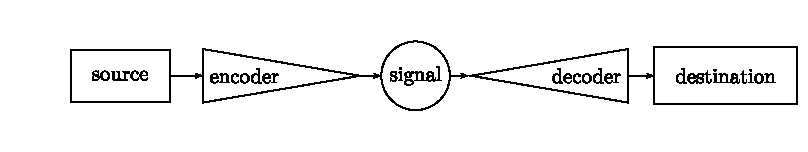
\includegraphics[width=1\textwidth,height=\textheight]{main_files/mediabag/figures/fig-process-comm.pdf}

}

\subcaption{\label{fig-schramm-schema-orig}コミュニケーションモデル
Communication model}

\end{minipage}%
\newline
\begin{minipage}{\linewidth}

\centering{

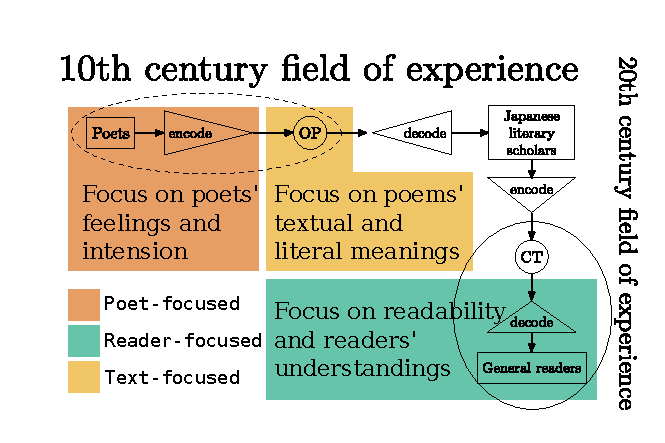
\includegraphics[width=1\textwidth,height=\textheight]{main_files/mediabag/figures/fig-schema-op-ct-tikz.pdf}

}

\subcaption{\label{fig-schramm-schema-adap}翻訳アプローチの分類とコミュニケーションモデルにおける位置づけ
Classification of Translation Approaches Based on the Communication
Model}

\end{minipage}%

\caption{\label{fig-schramm-schema}\textbf{コミュニケーションモデルから見る翻訳アプローチの分類
Classification of Translation Approaches Based on the Communication
Model}}

\end{figure}%

\subsection{追加率・不一致率の計算}\label{ux8ffdux52a0ux7387ux4e0dux4e00ux81f4ux7387ux306eux8a08ux7b97}

本稿では、訳における追加率は情報の補足の量を操作するものとし、原文における不一致率は原文の情報の欠落の量を操作するものとする。ノンリテラル情報の抽出は、追加率の高く、不一致率の低い訳が望ましい。そのため、追加率を客観的に調査し、このずれを明確にする必要がある。

追加率と不一致率の計算方法として、要素の順序や重複を考慮しない集合演算(バッグ法)と、要素の順序や重複を考慮するアライメント(整列法)を用いる。手順は、Yamamoto
(2005) と Yamamoto and Hodošček (2019)
でも説明されているが、詳細な手順は示されていなかったため、本稿では計算のプロセスをより明確にする。
Yamamoto (2005) と Yamamoto and Hodošček (2019)
のアプローチでは、語の複数の意味をメタコードで同時に保持し、不一致率の計算を行っている。デフォルトの分類語彙表番号、または複合語において一致語がある場合、その下位分解やその他の意味の一致可能性については考慮しない。このアプローチのメリットは、複合表現の一致を優先し、多義語のいずれかの意味が一致する可能性を計算に含めることにある。
計算において、重要な前提は、翻訳者が100\%の情報を翻訳に含めようとする努力を行っていると見なすことである。そのため、現代語に形式的に一致する語がない場合でも、原文のいずれかの要素と1対1で対応していると仮定し、追加率からその分を差し引く\footnote{これを純粋なアノテーション
  (pure annotation) と呼ぶ}。しかし、歌ことばに対応する語が明らかに存在しない場合、それは情報の欠落を訳者が認識していることを意味し、逐語訳の前提が理論的であることを示す。また、対応単位が変動するため、訳語の数のカウントが変わり、訳者ごとの追加率の比較が直感的でなくなることもある。
本稿では、追加率の計算手順を明確化し、結果の再現性を補足する。計算の調整は、当初の結論に影響を与えない。本稿の計算では、デフォルトの分類語彙表のメタコードと分解された最小単位を統一した上で実施する。\footnote{計算スクリプトは、他の選択肢も提供している。}

\paragraph*{旧分類語彙表番号(旧 WLSP
番号)に基づく一致の層づけ}\label{ux65e7ux5206ux985eux8a9eux5f59ux8868ux756aux53f7ux65e7-wlsp-ux756aux53f7ux306bux57faux3065ux304fux4e00ux81f4ux306eux5c64ux3065ux3051}
\addcontentsline{toc}{paragraph}{旧分類語彙表番号(旧 WLSP
番号)に基づく一致の層づけ}

歌ことばと現代語訳の「一致・不一致」は、以下のように4つのレベルに層づけされる。これは、二語のメタコード(旧
WLSP 番号)の最長共通部分列 (Longest Common Subsequence, LCS) (Sankoff
1972; Traum and Habash 2000) の長さによって決定される。

\[
\text{match}(s,t) \in
\begin{cases}
U, & \text{if } \text{LCS}(s,t) < 10 \\
G, & \text{if } 10 \leq \text{LCS}(s,t) < 13 \\
F, & \text{if } 13 \leq \text{LCS}(s,t) < 17 \\
E, & \text{if } \text{LCS}(s,t) \geq 17 \\
\end{cases}
\]

ここで、\(s\) はソーステキスト(和歌)の語のメタコード、\(t\)
はターゲットテキスト(現代語訳)の語のメタコードを表し、\(\text{LCS}(s,t)\)
は \(s\) と \(t\)
のメタコードの最長共通部分列の長さを示す。具体的な分類例を以下に示す。

\begin{enumerate}
\def\labelenumi{\arabic{enumi}.}
\tightlist
\item
  \textbf{Unmatch} (\(\text{match}(s,t) \in U\); \(\text{LCS}(s,t)=4\)):

  \begin{itemize}
  \tightlist
  \item
    \(s=\) \texttt{{[}BG-0{]}1-5520-20-0401} 梅 (plum)
  \item
    \(t=\) \texttt{{[}BG-0{]}8-0061-07-010-A} の (of, genitive case)
  \end{itemize}
\item
  \textbf{Group match} (\(\text{match}(s,t) \in G\);
  \(\text{LCS}(s,t)=11\)):

  \begin{itemize}
  \tightlist
  \item
    \(s=\) \texttt{{[}BG-01-5520-{]}20-0401} 梅 (plum)
  \item
    \(t=\) \texttt{{[}BG-01-5520-{]}19-115-A} 秋萩 (autumn bush clover)
  \end{itemize}
\item
  \textbf{Field match} (\(\text{match}(s,t) \in F\);
  \(\text{LCS}(s,t)=11\)):

  \begin{itemize}
  \tightlist
  \item
    \(s=\) \texttt{{[}BG-01-2030-01-{]}0300} 神 (god)
  \item
    \(t=\) \texttt{{[}BG-01-2030-01-{]}030-A} 仏 (Buddha)
  \end{itemize}
\item
  \textbf{Exact match} (\(\text{match}(s,t) \in E\);
  \(\text{LCS}(s,t)=17\)):

  \begin{itemize}
  \tightlist
  \item
    \(s=\) \texttt{{[}BG-01-5520-20-040{]}1} 梅 (plum)
  \item
    \(t=\) \texttt{{[}BG-01-5520-20-040{]}-A} 梅 (plum)
  \end{itemize}
\end{enumerate}

\paragraph*{バッグ法による不追加率の計算}\label{ux30d0ux30c3ux30b0ux6cd5ux306bux3088ux308bux4e0dux8ffdux52a0ux7387ux306eux8a08ux7b97}
\addcontentsline{toc}{paragraph}{バッグ法による不追加率の計算}

バッグ法を用いた追加率の計算は、現代語訳における和歌原文の追加要素を、順序関係を考慮せず、2つのテキストを集合と見なし、一致語の数から算出する。ソーステキスト(和歌)\(S=(s_i)_{i \in \mathbb{Z}^{+}}\)
とターゲットテキスト(現代語訳) \(T=(t_i)_{i \in \mathbb{Z}^{+}}\)
が与えられた場合、ターゲットテキストにおける追加率は以下の式で計算される。

\[
\begin{align}
\text{Addition Rate}(S,T) &= 1 - \frac{1}{|T|}\text{agreement}_{S}\\
\text{agreement}_{S}(S,T) &= \sum_{s_i \in S} \mathbb{I} \left( \exists t_j \in T \text{ such that } \text{match}(s_i, t_j) \notin U \right)
\end{align}
\]

\(\text{agreement}_{S}\)
は、ソーステキストにおいて一致語をもつトークンの数であり、\(\frac{1}{|T|}\text{agreement}_{S}\)
を一致率(バッグ法)と定義する。分母はターゲットテキストのトークン数
\(|T|\) である。\(s_i\), \(t_j\) はそれぞれソーステキストの \(i\)
番目と、ターゲットテキストの \(j\)
番目のトークンを意味する。追加率は、1から一致率を引くことで計算される。\(\mathbb{I}\)
は指示関数(indicator function)で、条件が真(\(s_i\)
が訳で一致語をもつ)の場合は1を、偽(\(s_i\)
が訳で一致語をもたない)の場合は0を返す。\footnote{ここでの一致率の計算は、\(\mathbb{I}\)
  内の条件で調整できる。今回は、メタコードが \(E, F, G\)
  のいずれかのレベルで一致する場合を一致と定義している。}

この計算において重要なのは、ソーステキストの語について、一致語があるかどうかをソーステキストの視点から判断することである。たとえターゲットテキストで複数の語がソーステキストの一語に対応しても、それらを一語と見なし、他の語を追加要素とする。この理由は、処理の一貫性を保つためである。たとえば、「散る」を「散り乱れる」と訳した場合、どこまでを一語と見なすかは曖昧であるため、「乱れる」を追加要素として扱う。つまり、計算では一対一の対応を前提としている。\footnote{なお、本稿のデータベースは、次の3つの基準を使った計算方法を提供している:短単位のみの計算、多義性を無視し複合単位を優先する計算、多義性の複合単位の構成要素をそのまま残す計算。今回は短単位を基準として計算を行う。}

不一致率についても同様に、ソーステキストに存在する要素のうち、ターゲットテキストで一致語が存在しない割合として計算する。この場合、分母はソーステキストのトークン数
\(|S|\) となる。

\[
\begin{align}
\text{Unmatch Rate}(S,T) &= 1 - \frac{1}{|S|}\text{agreement}_{S}
\end{align}
\]

バッグ法で算出された追加率をもとに、訳者の主観的な翻訳アプローチがどの程度影響を与えているかを統計的に検証する。また、不一致率については、初歩的な記述統計を用いて確認する。

\paragraph*{整列法による追加率・不一致率の計算}\label{ux6574ux5217ux6cd5ux306bux3088ux308bux8ffdux52a0ux7387ux4e0dux4e00ux81f4ux7387ux306eux8a08ux7b97}
\addcontentsline{toc}{paragraph}{整列法による追加率・不一致率の計算}

整列法による計算は、まずアライメント(整列)を推定し、次に整列された2語の一致数をもとに追加率を求める方法である。集合としてではなく、シーケンスとして順序を考慮する計算方法を用いる。

本稿では、分類語彙表番号を用いた動的計画法(Dynamic
Programming)に基づきアライメントを行う。動的計画法を用いて2つのシーケンス間のアライメントを計算するスコア関数は、以下のように定義される。

\[
\text{S}_{\text{DP}}(i, j) =
\begin{cases}
0 & \text{if } i = 0 \text{ or } j = 0 \\
\max
\begin{cases}
\text{S}_{\text{DP}}(i-1, j) - \text{gap} \\
\text{S}_{\text{DP}}(i-1, j-1) + \text{weight}(s_i, t_j) \\
\text{S}_{\text{DP}}(i, j-1) - \text{gap}
\end{cases} & i > 0 \text{ and } j > 0
\end{cases}
\]

このスコア関数 \(\text{S}_{\text{DP}}(i,j)\)
は、ソーステキストのシーケンス \(S\) とターゲットテキストのシーケンス
\(T\) の部分列の位置 \(i\) および \(j\)
までの最適なアライメントスコアを再帰的に計算するものである。重み付け関数
\(\text{weight}(s,t)\) は、LCS の値をそのまま使用し、Unmatch の場合は
\(-1\) のペナルティを与える(次式参照)。

\[
\text{weight}(s,t) =
\begin{cases}
-1, & \text{if } \text{match}(s,t) \in U \\
10, & \text{if } \text{match}(s,t) \in G \\
13, & \text{if } \text{match}(s,t) \in F \\
17, & \text{if } \text{match}(s,t) \in E \\
\end{cases}
\]

ギャップ(空白)の挿入には、ペナルティ (gap penalty) として \(0.01\)
を設定する。\footnote{和歌の翻訳では、語の対応が遠くなることが多いため、ギャップペナルティを
  \(0.01\) とすることで遠くの語の対応を許容している。}
この手法により、最も適したアライメントを探索する。整列後の例は以下の通りである。

\begin{verbatim}
>| 立田姫ーー手向けるーーーー神のあれ ばこそーーーーーーー秋の木の葉の幣ーーーと散るーーーらめー [298]
>| 竜田姫は、手向けをするべき神があるのでーーそのつかさどる秋の木の葉が幣のように散るのであろうよ [KBT]
\end{verbatim}

整列されたシーケンス \(S^{\prime}\) と \(T^{\prime}\)
を用いて、一致率と追加率を計算する。整列法による一致率と追加率の計算式は以下の通りである。

\[
\begin{align}
\text{Addition Rate}^{\prime}(S,T) &= 1-\frac{1}{|T|}\text{agreement}^{\prime}_{S}\\
\text{Unmatch Rate}^{\prime}(S,T) &= 1-\frac{1}{|S|}\text{agreement}^{\prime}_{S}\\
\text{agreement}^{\prime}_{S}(S,T) &= \sum_{s_i \in S^{\prime}} \mathbb{I} \left(\text{match}(s_i^{\prime}, t_i^{\prime}) \notin U \right)
\end{align}
\]

ここで、prime (\(\prime\))
記号がついているものは整列後のテキストを指す。指示関数 \(\mathbb{I}\)
は、アライメントで2語が一致する場合に1を返し、不一致の場合は0を返す。ギャップが含まれるアライメントは計算対象としない。また、一致率・不一致率・追加率の計算では、分母を整列前のソーステキストのトークン数に設定する。

動的計画法は、語順の変更や句の並び替えに対して弱いため、語順や句順が大きく異なる訳では、アライメントが適切に行えない場合がある。また、整列法は、アライメントされた2語が完全に一致するという厳しい前提があり、実際の翻訳状況とは異なることが多い。そのため、整列法で計算された追加率は、統計的な分析には用いず、個別のケーススタディで説明を行う。

\subsection{翻訳アプローチによる追加率の差の統計モデリング}\label{ux7ffbux8a33ux30a2ux30d7ux30edux30fcux30c1ux306bux3088ux308bux8ffdux52a0ux7387ux306eux5deeux306eux7d71ux8a08ux30e2ux30c7ux30eaux30f3ux30b0}

読者本位や歌人本位の訳文は、解釈や推論の追加が多く含まれる可能性が高く、ノンリテラル要素を多く抽出できると考えられる。しかし、訳者が主観的に読者本位・歌人本位のアプローチを意識しても、翻訳実践と翻訳アプローチの間にずれが生じることがある。各訳者が自身の翻訳アプローチにどれほど一貫しているかを、現代語訳の追加率と翻訳アプローチの関連の視点から検証する。翻訳アプローチによる追加率の差が統計的に見られない場合、和歌の翻訳実践に必然的に要素の追加が伴うことを意味すると考えている。先行研究
(Yamamoto 2005; Yamamoto and Hodošček 2019)
では、グループ・フィールド・同義レベルの一致率や、理論的・実験的追加率などの指標を計算しているが、翻訳者別の追加率の平均と標準偏差のみが提示されている。それぞれの値は訳者の意図・アプローチに沿った結果か、現代語訳において常なる結果かを調査する必要がある。

データの更新や計算手順の変更により、結果に変化が生じるため、新たに計算した追加率を対象に統計分析を行う。具体的には、翻訳アプローチ(\texttt{Focus})が追加率(\texttt{Addition\ Rate})に与える影響を検討するため、ベータ分布に基づく回帰モデルを採用する。ここでは、前述のバッグ法によって算出された追加率を応答変数として用いる。ベータ分布を用いる理由は、応答変数が
\((0, 1)\)
の範囲にあり、二項分布の代替として適しているためである。また、訳者(\texttt{Translator})と歌(\texttt{Poem\ ID})の変動を統制するためにランダム効果をモデルに含めている。モデルの詳細については補足資料を参照されたい。

モデルの推定には Markov Chain Monte Carlo (MCMC) 法を使用し、4
つのチェーンそれぞれで 2000 回のイテレーションを行い、そのうち 1000
回をウォームアップ (burn-in) とする。\texttt{R} (R version 4.3.3
(2024-02-29)) (R Core Team 2024) のパッケージ \texttt{brms} (2.21.0)
(Bürkner 2017) を使用してモデルを実装し、事後分布の収束は \(\hat{R}\)
指標および有効サンプルサイズ (ESS)
により評価する。モデルの推定結果として、各アプローチの追加率の事後分布をサンプリングし、中央値と
95\% の信用区間 (CrI) を報告する。なお、信用区間には事後最狭信用区間
(Highest Posterior Density Interval)
を用いる。また、アプローチ間の追加率の差についても、事後分布を示す。

事後分布の可視化と解釈は、Yu and Tamaoka (2020) の手法を参考とする。2
群の差の事後分布の 95\% CrI が 0 をカバーしているかを確認する。また、2
群の差が 0 より大きい確率も観測する。具体的には、95\% CrI が 0
をカバーしていない場合には 2 群の間に差があると判断し、0
をカバーしている場合でも、差が 0 より大きい確率が 95\%
より大きい、または 5\% より小さい場合には、傾向ありと認める。

\subsection{「立田」歌の事例分析}\label{ux7acbux7530ux6b4cux306eux4e8bux4f8bux5206ux6790}

現代語訳の和歌には、何らかの言い換えや追加が行われることがあるが、その要素の性質や内容が必ずしも明確ではない。これらの要素の性質を明らかにするため、アライメントにおける一致を確認しつつ、コーパス言語学の観点から分析を行う。本稿では、Sinclair
(1996)
の拡張意味単位モデルを参考にし、和歌の原文に見られるコーパスレベルの傾向が、対訳文のセンテンスレベルでどのように処理されているかを明らかにする。
拡張意味単位モデルは、コロケーション(collocation;
他の語の共出現関係)(Sinclair, Jones, and Daley 1970,
15)、コリゲーション(colligation;
構文パターンや文法的要素との共出現関係)(cf., Firth 1968, 183; Sinclair
1996, 11; 2003, 171)、意味的志向(semantic preference;
特定の意味の語群との共出現関係)(Sinclair 2003,
178)、そして談話韻律(discource prosody;
拡張意味単位全体の評価・態度・語用論的意味)(Sinclair 2004, 174)の 4
つのレベルで対象言語単位を記述する。このモデルにおいて、コロケーションから談話韻律へと進むにつれて、直接的な観測が難しくなり、明示的ではなくなる
(Stubbs 2001, 87--88)。
和歌の性質とデータの量が少ないため、すべての拡張意味単位を正確に捉えることは困難である。したがって、本稿では、拡張意味単位の
4 つのレベルを 4
つの視座として、それぞれ共出現の語、構文パターン、語の意味的まとまりについて、10
人の翻訳者がどのように処理しているかを分析する。

Yamamoto (2005) では、現代語訳の紹介に歌枕「立田」の歌 298
番をとりあげている。本稿でも同じ歌をとりあげ、それが 10
人の翻訳、異なる翻訳の方針でどのように処理されているか、前掲の 3
つの視座から分析する。

コロケーションのレベルで確認すると、八代集全体における 54 首において、
「立田」の文脈に頻出する内容語
\footnote{形態素解析システム Chasen を用いたため、Chasen の ID が 60
  以前のもの}には「山」(30;うち共出現語として 15
あり、「立田山」の複合表現として 15
ある)「紅葉づ」(17)「川」(「立田川」の複合表現として 15
ある)「秋」(15)「見る」(12)「紅葉葉」(9)「錦」(9)
があげられる。
頻度5以上の語には、「神無備」(5)「姫」(うち「立田姫」の複合表現として
8 ある)
など神に関連する語と、「散る」(8)「流る」(5)「吹く」(6)「紅葉」(5)「黄葉」(5)
など、落葉に関連する語が存在している。\footnote{詳細は補足資料を参照されたい。}

共出現する構文パターンとして、動詞の終止形で終わる歌の少なさ(古今集 12
首の中で 1 首のみ)が観測される。また、古今集の中では、係り結びは 9
首観測されており、
余韻の残し方に特徴があると考えられる。これら終わり方の構文パターンが、翻訳における処理について考察する。

共出現する語の性質は、内容語のコロケーションは基本的に、「立田川」「立田(の)山」など地名を構成する「山」「川」のグループのほか、秋の「神」に関連する関連語のグループが明瞭に見える。神聖なる場所の歌枕の性質が伺える。

298
番歌の訳における追加要素のバリエーションを示しながら、以上のコーパスレベル・大局レベルの要素が
298
番歌のセンテンスレベルで組み込まれるか、どのように組み込まれているかを確認し、ノンリテラル要素と捉えられるかを論じる。

\section{結果}\label{sec-results}

\subsection{現代語訳の整理と分類}\label{ux73feux4ee3ux8a9eux8a33ux306eux6574ux7406ux3068ux5206ux985e}

注釈書の前書きや導入部に記されている翻訳アプローチに関する意識と認識に基づき、10
人の翻訳者のアプローチをコミュニケーションの主体に対する視座の置き方によって、以下の
3 類に分類した。

\begin{enumerate}
\def\labelenumi{\arabic{enumi}.}
\item
  \textbf{テキストの字義を重視する方針}: 金子 (1933), 窪田 (1960), 片桐
  (1998)
\item
  \textbf{作者の意図を重視する方針}: 奥村 (1978), 竹岡 (1976)
\item
  \textbf{読者の理解を重視する方針}: 小沢 (1971), 久曽神 (1979)
\end{enumerate}

ただし、松田 (1968), 小島 and 新井 (1989), 小町谷 (1982)
は、明確に翻訳アプローチについての記述がなかった。

テキストの字義を重視する翻訳アプローチは、逐語訳に最も忠実である。一方、作者の意図や感受性を重視するアプローチおよび読者の理解を重視するアプローチでは、語や語順の入れ替えや、語句の補いを一定程度許容していることが示唆されている。

\subsubsection*{Text-focused approach: KNK, KBT,
KTGR}\label{text-focused-approach-knk-kbt-ktgr}
\addcontentsline{toc}{subsubsection}{Text-focused approach: KNK, KBT,
KTGR}

原文の字義通りの解釈を重視する訳のグループは、原文に忠実な翻訳を行い、可能な限り語順や意味を変えずに訳すことに重点を置くものである。例えば、金子
(1933)
は「逐語訳」を徹底し、語の追加や削除を避け、慎重に翻訳を行っていると述べている。また、金子
(1933)
は、歌の意味を損ねたり調子を誤ったりすることを恐れ、鏡花水月の訳法\footnote{あからさまに説明せず、ただその姿を眼前に思い浮かべるようにする漢文の表現法}
にしたがい、一字一語の変更を許さない慎重な翻訳方針を採っている。文体面では、例えば「くずをれる」といった古風な言葉をあえて用いるなど、本居宣長の『遠鏡』に似た翻訳調を採用している。

窪田 (1960)
も、現代語訳の方針として逐語訳にこだわり、語順の変更や新しい語の追加を避けていると述べている。同様に、片桐
(1998)
も逐語訳を行い、和歌の省略や過度な補足を避け、可能な限り忠実に現代語訳を実施していると述べている。

\subsubsection*{Poet-focused approach: OKMR,
TKOK}\label{poet-focused-approach-okmr-tkok}
\addcontentsline{toc}{subsubsection}{Poet-focused approach: OKMR, TKOK}

歌人の作意を重視する訳のグループは、表面的な意味よりも原文の意図と感受性を重視するグループである。奥村
(1978, 7)
は「口語訳は、原歌の言葉遣いや言い回しを尊重し、一首の意味を厳密に解釈するよりも、基本的な作意をまず感じ取ってもらうことに重点を置いた」と述べている。原文の意図の理解を重視し、逐語訳よりも作意を優先して翻訳を行っている。竹岡
(1976, 上下:21)
は、訳(口語訳)は原文の「筋」の紹介や解説の類ではなく、作者の認識の仕方や感じ方をあらゆる面から明らかにしたのち、それを現代語に存在する同じ、あるいは極力それに近い認識の仕方や感じ方の表現に忠実に置き換えることを指している。つまり、表面的には原歌の同義語に拘るものの、原歌における歌人の感受性の保持に重点を置いている。

具体的な現代語訳の方針として、竹岡 (1976, 上下:11-\/--12)
は次のような独自の理論を提案している。

\[
S=\left[\left(a+b+c+\dots+n\right)\times X \right]\times Y
\]

\(S\) は翻訳された歌であり、\(a, b, c, \dots, n\)
のそれぞれは歌における語、\(X\) は訳に含まれる要素であり、\(Y\)
は訳に効果的に加えられた要素である。\(a, b, c, \dots, n\)
それぞれの一般的普遍的意義は辞書で理解でき、それぞれの \(+\)
の仕方に相当するものは文法書を参照すれば理解できるとしている。竹岡
(1976, 上下:11) は、\(Y\) は通常は 0
の値であるが、和歌にはいくつか効果的な要素が含まれる時、翻訳者は \(Y\)
に何らかの値、例えば終助詞(わ、ね、よ)を付け加える。したがって、現代語訳作成のための重要な変数は
\(X\) となる。その \(X\)
は、語句の分割、対応する適切な現代語、語順、助詞・接続詞を含めた訳語、文の構造、話の流れ(談話)、場面の7つに分類されるとしている。このように、歌の筋よりも作者の意図を細部まで還元することを強調していると解釈できる。\footnote{契沖の「古今和歌集余材抄」以来の7種の注釈書の注を統合した初めてのものである。竹岡はこの注釈書にて文学研究に分析的アプローチを組み込んでいる。竹岡は賀茂真淵、香川景樹の仕事を分析に根拠がないとして同意できないとする一方で、契沖、本居宣長、富士谷成章(1738--79)らの注釈を評価している。加えて、特に古典文法、語彙の観点から7種すべての古注間の違いについて慎重に議論している。}

\subsubsection*{Reader-focused approach: OZW,
KSJ}\label{reader-focused-approach-ozw-ksj}
\addcontentsline{toc}{subsubsection}{Reader-focused approach: OZW, KSJ}

読者の理解を重視する訳のグループは、原文に忠実であることよりも、読者の内容の理解や解釈を読者に伝えることを重視している。そのため、語順を変えたり、新しい語を加えることもある。
小沢 (1971)
は原作の語順・語法を変更することをいとわず、読者が理解しやすいように内容を優先した翻訳を行っている。
小沢 (1971, 46)
は「口語訳はそれだけ独立しても意味がよくわかるように努めたので、時には原作の語順・語法を変えている」と述べており、逐語訳よりも内容の理解の方に力点が置かれている。久曽神
(1979)
は、平易な口語訳を採用し、必要に応じて語句を補っており、解釈を重視した翻訳を行っている。現代語訳の方針としては「歌意は、歌句に基づく平易な口語訳としたが、必要と思われる場合は字句を補った」と述べている
(久曽神 1979, 1--5:6)。

\subsubsection*{その他のアプローチ: KMCY, MTD,
K\&A}\label{ux305dux306eux4ed6ux306eux30a2ux30d7ux30edux30fcux30c1-kmcy-mtd-ka}
\addcontentsline{toc}{subsubsection}{その他のアプローチ: KMCY, MTD,
K\&A}

現代語訳の方針について、小町谷 (1982)、松田 (1968)、小島 and 新井 (1989)
は明確に述べていない。

うち、松田 (1968)
の現代語訳は、他の10名の共同執筆者によって作成されている。この注釈書の冒頭で述べられている解説によれば、現代語訳はこれまでの研究に基づいて作成されたとしているが、10名の共著者の間で翻訳の共通認識や作成方針については明確に述べられていない。また、松田は古今集の和歌について、歌人の感情だけでなく、選者の編集意識も解釈に含めようとしていると述べている
(松田 1968, 上下:9)。

小島 and 新井 (1989)
の特色の一つは、注釈に江戸期(1600--1868)だけでなく、それまでの注釈書では無視されてきた中世期(1392--1600)に作られた注釈も取り入れていることである
{[}pp.~481--482{]}。また、万葉集の和歌と用語を対比して引用している (小島
and 新井 1989,
480)。各歌の注釈は、「歌番号」「大意」「語句の注」「参考事項」の順で述べられており、他の注釈本と比べて量的にはさほど違いはないが、付録には多様な資料が含まれており、その分量は本全体の30\%を占めている。

\subsubsection*{まとめ}\label{ux307eux3068ux3081}
\addcontentsline{toc}{subsubsection}{まとめ}

それぞれの翻訳アプローチを見る限り、ほとんどの作者が逐語訳を基本とし、原文の意味を変えない翻訳を試みているが、従来の注釈書の継承の仕方や情報伝達における重点の置き方には違いが見られる。本稿では、「テキストの字義を重視」「作者の意図・感受の解釈を重視」「読者の理解を重視」「その他」というコミュニケーションモデルの観点から分類を行った。この中で、原文の字義を重視する翻訳アプローチは、最も逐語訳にこだわっていた。作者の意図や感受を重視する、または読者の理解を重視する翻訳アプローチでは、語順や語句の多少の入れ替えや補いを許容していた。ただし、この分類には重なり合う部分もあると考えられる。

\subsection{不一致率と追加率の推定結果}\label{ux4e0dux4e00ux81f4ux7387ux3068ux8ffdux52a0ux7387ux306eux63a8ux5b9aux7d50ux679c}

追加率の計算結果を Figure~\ref{fig-data} に示す。不一致率は 0--88 \%
の範囲であった Table~\ref{tbl-data-review}。中でも、TKOK
の現代語訳が最も不一致率が低く、17.2 \% (sd = 0.1) であった
Figure~\ref{fig-unmatch-rate}。一方、OZW の現代語訳が最も高く、23\% (sd
= 0.112) であった Figure~\ref{fig-unmatch-rate}。既に述べたように、OZW
は語順を変更することをいとわないのに対し、竹岡は自身の方針に忠実に翻訳を行っている。この差がデータに明確に表れていると言える。

10 種の現代語訳のうち、697番歌は不一致率が 88.2\% と最も高い和歌であった
Table~\ref{tbl-data-review}。つまり、和歌の中のほとんどの語が訳されていないことを示している。このような歌については、次の例で確認する。

\begin{figure}

\centering{

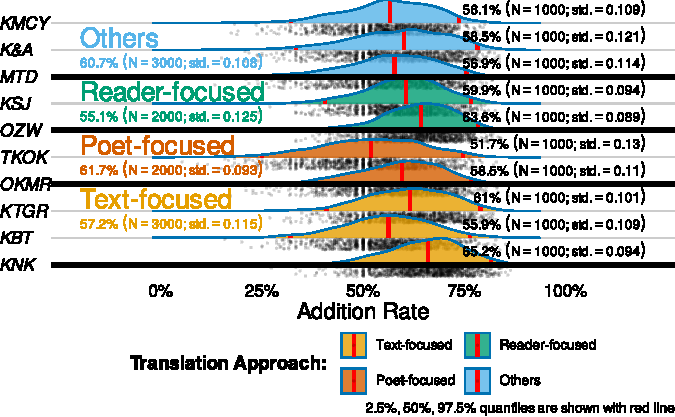
\includegraphics{main_files/mediabag/main_files/figure-pdf/fig-data-1.pdf}

}

\caption[訳者別の追加率の確率分布]{\label{fig-data}訳者別の追加率の確率分布
Probability distribution of addition rates by translator}

\end{figure}%

\begin{verbatim}
Picking joint bandwidth of 0.0242
\end{verbatim}

\begin{figure}

\centering{

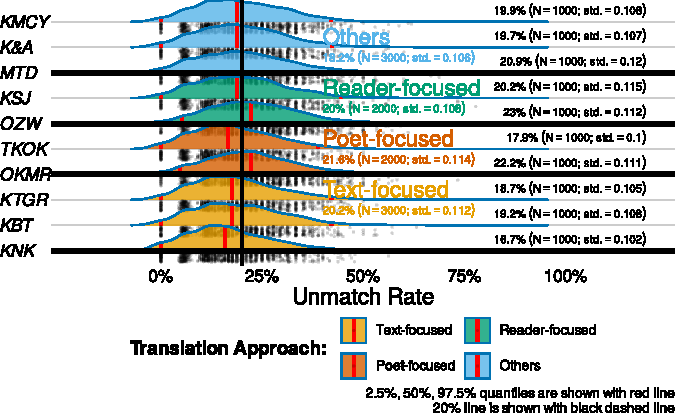
\includegraphics{main_files/mediabag/main_files/figure-pdf/fig-unmatch-rate-1.pdf}

}

\caption[不一致率(明確な対応をもたない要素が和歌原文を占める割合)の概要]{\label{fig-unmatch-rate}訳者別の不一致率の確率分布(明確な対応をもたない要素が和歌原文を占める割合)
Probability distribution of unmatch rates by translator (unmatch rate is
the proportion of elements in the original poem without agreement)}

\end{figure}%

\begin{table}

\caption{\label{tbl-data-review}不一致率・追加率の概要 Summaries of
unmatch and addition rates}

\begin{minipage}{\linewidth}

[!h]
\centering
\begin{tabular}{l|r|r|r|r|r}
\hline
 & 最小値\Min. & 最大値\Max. & 中央値\Median & 平均値\Mean & 標準偏差\sd\\
\hline
不一致率 (Unmatch Rate) & 0.000 & 0.882 & 0.188 & 0.198 & 0.110\\
\hline
追加率 (Addition Rate) & 0.053 & 0.864 & 0.600 & 0.587 & 0.114\\
\hline
\end{tabular}

\end{minipage}%
\newline
\begin{minipage}{0.45\linewidth}

[!h]
\centering
\begin{tabular}{l|l|r}
\hline
訳者\Translator & 歌番\Poem ID & 不一致率\Unmatch Rate\\
\hline
MTD & 697 & 0.882\\
\hline
KSJ & 404 & 0.778\\
\hline
KSJ & 886 & 0.733\\
\hline
OKMR & 515 & 0.733\\
\hline
KSJ & 515 & 0.733\\
\hline
\end{tabular}

\end{minipage}%
%
\begin{minipage}{0.10\linewidth}
~\end{minipage}%
%
\begin{minipage}{0.45\linewidth}

[!h]
\centering
\begin{tabular}{l|l|r}
\hline
訳者\Translator & 歌番\Poem ID & 不一致率\Unmatch Rate\\
\hline
KNK & 880 & 0.864\\
\hline
OKMR & 736 & 0.857\\
\hline
KNK & 705 & 0.857\\
\hline
KNK & 868 & 0.854\\
\hline
KNK & 364 & 0.851\\
\hline
\end{tabular}

\end{minipage}%
\newline
\begin{minipage}{0.45\linewidth}

[!h]
\centering
\begin{tabular}{l|r|r}
\hline
歌番\Poem ID & 平均値\Mean & 標準偏差\sd\\
\hline
718 & 0.481 & 0.078\\
\hline
703 & 0.472 & 0.109\\
\hline
576 & 0.467 & 0.070\\
\hline
150 & 0.447 & 0.084\\
\hline
515 & 0.440 & 0.164\\
\hline
\end{tabular}

\end{minipage}%
%
\begin{minipage}{0.10\linewidth}
~\end{minipage}%
%
\begin{minipage}{0.45\linewidth}

[!h]
\centering
\begin{tabular}{l|r|r}
\hline
歌番\Poem ID & 平均値\Mean & 標準偏差\sd\\
\hline
669 & 0.773 & 0.046\\
\hline
420 & 0.773 & 0.065\\
\hline
705 & 0.771 & 0.052\\
\hline
749 & 0.768 & 0.052\\
\hline
143 & 0.767 & 0.059\\
\hline
\end{tabular}

\end{minipage}%

\end{table}%

\subsubsection*{不一致率の高い対訳}\label{ux4e0dux4e00ux81f4ux7387ux306eux9ad8ux3044ux5bfeux8a33}
\addcontentsline{toc}{subsubsection}{不一致率の高い対訳}

不一致率の高い歌の対訳において、10人の現代語訳に共通して欠落が見られたのは「序詞」「枕詞」「まわりくどい言い回し」の3種類であった。訳者の一部は、意識的に「序詞」や「枕詞」を訳さずに省略していることが観測された。例えば、松田
(1968) の現代語訳では、4首が原文よりも短くなっている。MTD (173) と MTD
(665) の訳では、枕詞「ひさかたの」「みつしほの」が省略されている。MTD
(684) および MTD (697)
の訳においては、枕詞も序詞も省略されている。これらの歌は当然不一致率も高く、特に
MTD (697) は原文よりも著しく短くなっている\footnote{KSJ (404)
  もまた極端に短く、序詞が省略されている。}。MTD (697)
では、大和の枕詞「敷島の」が省略されている。原文では「頃も」と「衣」が掛詞になっているが、その「衣」に掛かる序詞も省略されている。

\begin{figure}

\centering{

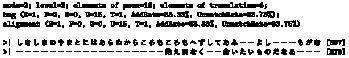
\includegraphics[width=1\textwidth,height=\textheight]{main_files/mediabag/figures/matsuda-697.pdf}

}

\caption{\label{fig-mtd-697}697番歌の 松田 (1968)
による現代語訳:アライメントの結果を書き換えている;「しきしまのやまとにはあらぬからころも」が省略されている。Contemporary
translation of Poem \#697 by 松田 (1968): The alignment has been
revised; the \emph{jokotoba} ``Shikishima no Yamato ni wa aranu kara
koromo'' has been omitted.}

\end{figure}%

和歌と現代語訳の間に見られるまわりくどい表現の不一致は、翻訳における「欠落」というよりも、本稿の一致の探し方(アルゴリズムとして一対一で探索する)に課題があると言えるが、一例を挙げる。OKMR
(\#346)
において、奥村の現代語訳は和歌の語をほとんど使用せず、あえて次のようにまわりくどい表現を用いている:

\begin{itemize}
\tightlist
\item
  「とりそへて」=「さらにそえて」
\item
  「とどめおきて」=「のこしておきましょう」
\end{itemize}

特に整列法は、このような歌をうまくアライメントできなかった。

\subsubsection*{追加率の高い対訳}\label{ux8ffdux52a0ux7387ux306eux9ad8ux3044ux5bfeux8a33}
\addcontentsline{toc}{subsubsection}{追加率の高い対訳}

MTD (\#629)
は追加率が高い訳のひとつである。この歌には「あやなし」「まだき」などの古語や、「なくに」のような現代語では使われない語法が含まれている。これらの語は、現代語と分類語彙表番号で対応づけることができなかった。また、「名の\textbf{たつ}」と「\textbf{たつ}たがは」の掛詞も存在する
Figure~\ref{fig-mtd-629}。

追加率の平均値が上位の 10 首のうち、他にも 705 番歌、669 番歌、617
番歌など、追加率の高い和歌が含まれている。705
番歌には「身」と「雨」に「降(経)る」の掛詞が含まれている。669 番歌と
617
番歌には、それぞれ「海藻目」と「ながめ」の掛詞がある。掛詞を含む歌が典型的であった。

\begin{figure}

\centering{

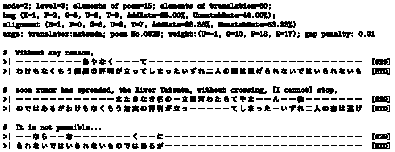
\includegraphics[width=1\textwidth,height=\textheight]{main_files/mediabag/figures/matsuda-629.pdf}

}

\caption{\label{fig-mtd-629}629 番歌の 松田 (1968)
による現代語訳:アライメントの結果を書き換えている Contemporary
translation of Poem \#629 by 松田 (1968): The alignment results have
been modified.}

\end{figure}%

\subsection{翻訳アプローチによる追加率の差}\label{ux7ffbux8a33ux30a2ux30d7ux30edux30fcux30c1ux306bux3088ux308bux8ffdux52a0ux7387ux306eux5dee}

本節では、統計モデリングを用いて翻訳アプローチによる追加率の差を検証する。モデルが推定した効果のいずれの
\(\hat{R}\) も 1 であり、1.1 を下回って収束が良好であることが示された
(Brooks and Gelman 1998)。検証対象の効果について、ESS はすべて 2000
程度に達した。

\subsubsection*{翻訳アプローチによる追加率の相違が小さい}\label{ux7ffbux8a33ux30a2ux30d7ux30edux30fcux30c1ux306bux3088ux308bux8ffdux52a0ux7387ux306eux76f8ux9055ux304cux5c0fux3055ux3044}
\addcontentsline{toc}{subsubsection}{翻訳アプローチによる追加率の相違が小さい}

Figure~\ref{fig-poster}
は翻訳アプローチごとの追加率の事後分布を示している。この図から以下の情報が得られた。

\begin{enumerate}
\def\labelenumi{(\alph{enumi})}
\item
  追加率は、翻訳アプローチにかかわらず、現代語訳の要素の約 50\%
  が追加的な要素であることがわかった。この点は観測データからも確認されている。
\item
  翻訳アプローチグループ間で比較した結果、2 グループ間の差の事後分布の
  95\% CrI はすべて 0 を含んでおり、それぞれの 2
  グループの追加率に有意な差は認められなかった。傾向としては、\texttt{Reader-focused}
  群の追加率に比べ、\texttt{Other} 群の追加率が \(-4\%\) 程度下回った
  (\(\mathrm{posterior\; median} = -0.04\%; 95\%\;\mathrm{CrI} = [-0.13, 0.05]\),
  \(P(\Delta>0) = 14\%\))。また、\texttt{Reader-focused} 群の追加率は
  \texttt{Poet-focused} 群よりも \(6\%\) 程度下回った
  (\(\mathrm{posterior\; median} = 0.06\%; 95\%\;\mathrm{CrI} = [-0.03, 0.16]\),
  \(P(\Delta>0) = 91.6\%\))
  ことが観測されているが、傾向差の基準には達しなかった。
\end{enumerate}

\begin{figure}

\centering{

\centering{

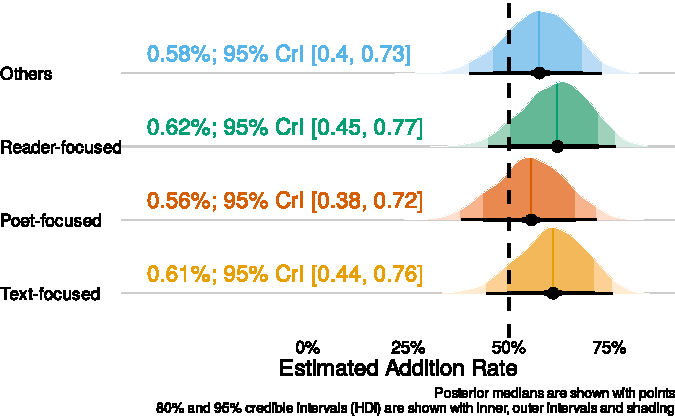
\includegraphics{main_files/mediabag/main_files/figure-pdf/fig-poster-1.pdf}

}

\subcaption[追加率の事後分布]{\label{fig-poster-1}各翻訳アプローチの追加率の事後分布
Posterior distribution of addition rates for each translation approach}

\centering{

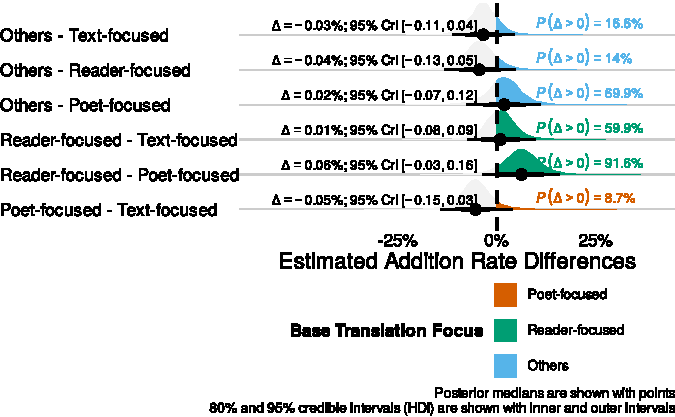
\includegraphics{main_files/mediabag/main_files/figure-pdf/fig-poster-2.pdf}

}

\subcaption[追加率の事後分布]{\label{fig-poster-2}翻訳アプローチによる追加率の差の事後分布
Posterior distribution of differences in addition rates by translation
approach}

}

\caption{\label{fig-poster}追加率の事後分布 Posterior distribution of
addition rates}

\end{figure}%

\subsubsection*{訳者による追加率の変動より歌による変動のほうが大きい}\label{ux8a33ux8005ux306bux3088ux308bux8ffdux52a0ux7387ux306eux5909ux52d5ux3088ux308aux6b4cux306bux3088ux308bux5909ux52d5ux306eux307bux3046ux304cux5927ux304dux3044}
\addcontentsline{toc}{subsubsection}{訳者による追加率の変動より歌による変動のほうが大きい}

階層モデリングにおいて、訳者と歌をランダム切片としてモデル化している。訳者グループと歌グループがそれぞれ共有していると仮定した正規分布のパラメータである標準偏差の事後分布を可視化した
Figure~\ref{fig-hyperparameter}。訳者グループの標準偏差の分布は、歌グループの標準偏差の分布よりも左寄りであった。これは、訳者間の変動よりも歌間の変動のほうが大きいことを示している。つまり、ランダム効果の視点から見ると、歌が訳者に比べて追加率の変動により大きく寄与していると考えられる。

\begin{figure}

\centering{

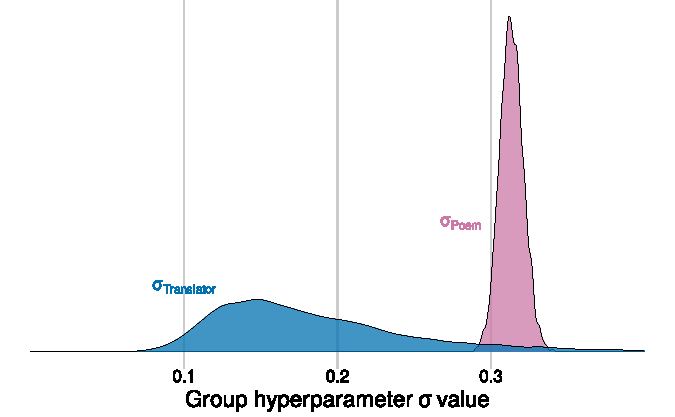
\includegraphics{main_files/mediabag/main_files/figure-pdf/fig-hyperparameter-1.pdf}

}

\caption[グループレベルのハイパーパラメータの事後分布]{\label{fig-hyperparameter}グループレベルのハイパーパラメータの事後分布
Posterior distribution of group-level hyperparameters}

\end{figure}%

\subsection{298
番「立田」歌の訳の事例分析}\label{ux756aux7acbux7530ux6b4cux306eux8a33ux306eux4e8bux4f8bux5206ux6790}

298 番「立田」の歌についての事例分析は、アライメントを示しながら進める。

298
番歌の不一致率および翻訳における追加率のまとめは、Table~\ref{tbl-tatsuta-review}
に示している。ここでの計算は整列法の結果に基づいている。歌のトークン数
19 のうち、アライメントで一致する 2 語対の数が OZW を除いて 14
を超えた。OZW
は文の入れ替えを行っているため、アライメントがうまく行われなかった。原文の要素の不一致率は低い水準に保たれており、訳における追加率は
OZW を除くと 50\% から 70\% となっていた。1 語あたり 1.5 から 1.7
語で訳されていた。アライメントはプログラムの出力を修正した上で
Figure~\ref{fig-alignment}
に整理している。修正前の出力については補足資料を参照されたい。さて、どのような追加要素があるか確認していく。

\begin{table}

\caption{\label{tbl-tatsuta-review}「立田」歌 298
番の現代語訳の不一致率・追加率の概要 Summary of unmatch and addition
rates in contemporary translations of ``Tatsuta'' Poem}

\centering{

[!h]
\centering
\begin{tabular}{l|l|l|r|r|r}
\hline
訳者\Translator & 歌番\Poem ID & 計算手法\Method & 一致数\Agreement Count & 不一致率\Unmatch Rate & 追加率\Addition Rate\\
\hline
KNK & 298 & Alignment & 17 & 0.105 & 0.691\\
\hline
KTGR & 298 & Alignment & 16 & 0.158 & 0.568\\
\hline
K&A & 298 & Alignment & 15 & 0.211 & 0.500\\
\hline
KMCY & 298 & Alignment & 17 & 0.105 & 0.622\\
\hline
KBT & 298 & Alignment & 15 & 0.211 & 0.500\\
\hline
KSJ & 298 & Alignment & 16 & 0.158 & 0.628\\
\hline
MTD & 298 & Alignment & 14 & 0.263 & 0.562\\
\hline
OKMR & 298 & Alignment & 14 & 0.263 & 0.682\\
\hline
OZW & 298 & Alignment & 7 & 0.632 & 0.851\\
\hline
TKOK & 298 & Alignment & 16 & 0.158 & 0.500\\
\hline
\end{tabular}

}

\end{table}%

\begin{figure}

\begin{minipage}{\linewidth}

\centering{

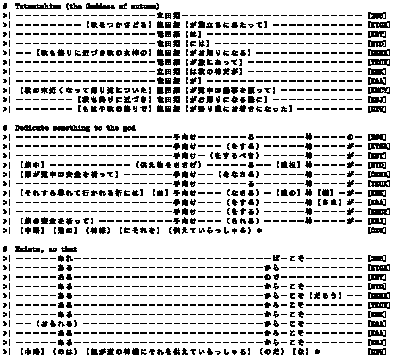
\includegraphics[width=1\textwidth,height=\textheight]{main_files/mediabag/figures/tatsuta-1.pdf}

}

\subcaption{\label{fig-alignment-1}アライメント(前半):たつたひめ
手向ける神の あればこそ Alignment (first half): Tatsutahime tamukeru
kami no areba koso `(There is) the god exits for Tatsutahime to dedicate
(things), so that \ldots{}'}

\end{minipage}%
\newline
\begin{minipage}{\linewidth}

\centering{

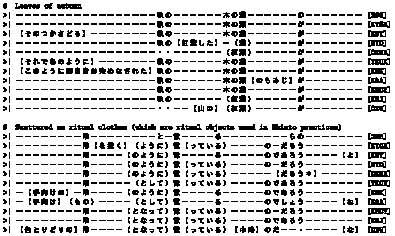
\includegraphics[width=1\textwidth,height=\textheight]{main_files/mediabag/figures/tatsuta-2.pdf}

}

\subcaption{\label{fig-alignment-2}アライメント(後半):秋の木の葉の
幣と散るらめ Alignment (second half): aki no konoha no nusa to chiru
rame `leaves of autumn may be scattered as ritual clothes (which is
dedicated to the god)'}

\end{minipage}%

\caption{\label{fig-alignment}10人の訳者のアライメント(筆者がアライメント推定プログロムの出力を修正して作成):「【】」は追加と判断する要素である;「()」は言い換えと判断する要素である。「*」は、句の順序の入れ替えで対応しうる文・語である。「・」は直訳されていないと判断する要素のプレースホルダーである。
Alignment of translations by 10 translators (the author corrected the
output of the alignment estimation program): Elements in ``【】'' are
judged as additions, those in ``( )'' are considered paraphrases,
``*'' indicates phrases or words aligned through sentence reordering,
and ``・'' represents elements judged not to be translated directly.}

\end{figure}%

\paragraph*{共出現語の訳出}\label{ux5171ux51faux73feux8a9eux306eux8a33ux51fa}
\addcontentsline{toc}{paragraph}{共出現語の訳出}

「立田」に関連するコーパスレベルの共出現語として、「山」「川」「紅葉づ」「姫」「手向く」「紅葉葉」「神無備」「秋」「幣」「散る」などが頻出する。298
番歌は、典型的な「立田」の歌として「姫」「手向く」「幣」「秋」を含んでおり、これらの語のほとんどがそのまま訳出されている。298
番歌には出現しない「紅葉葉」や「紅葉づ」は、「木の葉」を通じて暗示され、以下のように訳出されている:

\begin{itemize}
\tightlist
\item
  紅葉した葉 {[}MTD{]}
\item
  木の葉のもみじ {[}K\&A{]}
\item
  紅葉 {[}KSJ, OZW, OKMR{]}
\end{itemize}

一方、KBT、TKOK、KNK、KMCY、KTGR
は「このは」についての処理を行わなかった。

また、コーパスレベルの共出現語である「幣」については、以下のような追加が見られた:

\begin{itemize}
\tightlist
\item
  【色とりどりの】幣 {[}OZW{]}
\item
  【手向けの】幣 {[}KNK{]}
\item
  幣【を撒く】(ように)散(っている) {[}KTGR{]}
\end{itemize}

ただし、これらの追加が「立田」に帰属するべきかの判断は難しく、「幣」を介して間接的に情報を示すものと考えられる。

基本的に、コーパスレベルにおける「立田」の共出現要素の処理は、そのまま残す方針か、他の要素よりも多く追加する方針のいずれかとなっていることが伺える。また、「このは」のような共出現語ではない要素についても、全体的なコロケーションを考慮して「紅葉」として訳出されるケースが見られた。訳出の方針は、訳者にかかわらず安定的な翻訳が行われている。

訳と原文の差分から、コーパスレベルの共出現語に関連する重要な情報が見えてくると推測できる。

\paragraph*{構文パターンの訳出}\label{ux69cbux6587ux30d1ux30bfux30fcux30f3ux306eux8a33ux51fa}
\addcontentsline{toc}{paragraph}{構文パターンの訳出}

共出現する構文パターンとして、終止形で終わる歌の少なさ(古今集の12首のうち1首のみ)が観測されている。特に、古今集では12首中9首が係り結びを用いている。これらの文の終わり方などの構文パターンについて、298番歌の訳における処理を分析した。

298番歌の係り結びは、強意の「こそ」と推量の「らむ」の活用形「らめ」で構成されていた。その訳として、10人の訳者のうち7人が「こそ」を残しており、さらに9人が文末において「強調」の「ノ
{[}であろう・でしょう{]}」構文を使用している。推量の「らむ」についても、9人が「だろう・でしょう」と訳している。唯一「だろう」で訳していない
OZW は「だな」という詠嘆的な口調で訳している。KBT と K\&A
は文末にそれぞれ「よ」と「ね」の終助詞を追加している。

これらの構文パターンの訳出は、非常にロバストであることが確認できた。他の係り結びを使わない「立田」の歌の翻訳においても、この構文パターンが干渉して追加されているかを確認したが、該当する事例は見られなかった。つまり、特徴的な共出現の構文パターンの処理は、少なくとも「立田」の場合においては直訳に留まっている。

その他の文法的な要素として、格助詞の「と」や動詞の基本形式「-u」(例えば「なる」)の訳は、コーパスレベルにおいては「立田」の特徴的な共出現要素ではないが、分析を行った。その結果、以下のように多様な訳し方が確認された。

{[}\ldots 幣{]}「\textbf{と}」:

\begin{itemize}
\tightlist
\item
  {[}\ldots 幣を撒く\textbar 幣の{]}\textbf{ように} {[}KTGR, KBT, MTD,
  OKMR, KNK{]}
\item
  {[}\ldots 幣\textbar 手向けもの{]}\textbf{として} {[}TKOK, K\&A{]}
\item
  {[}\ldots 幣{]}\textbf{となって} {[}KMCY, KSJ, OZW{]}
\end{itemize}

{[}\ldots 散{]}「\textbf{る}」

\begin{itemize}
\tightlist
\item
  {[}\ldots 散っ{]}\textbf{ている} {[}KTGR, MTD, OKMR, TKOK, KMCY, KSJ,
  OZW{]}
\item
  {[}\ldots 散{]}\textbf{る} {[}KBT, KNK, K\&A{]}
\end{itemize}

{[}\ldots 手向け{]}「\textbf{る}」

\begin{itemize}
\tightlist
\item
  {[}\ldots 手向けを{]}\textbf{する} {[}KTGR, K\&A, KMCY{]}
\item
  {[}\ldots 供え物をささげ\textbar 手向け{]}\textbf{る} {[}MTD, TKOK{]}
\item
  {[}\ldots 手向けを\textbar お手向け{]}\textbf{なさる} {[}OKMR, KNK{]}
\item
  {[}\ldots 手向けを{]}\textbf{するべき} {[}KBT{]}
\item
  {[}\ldots 手向け{]}\textbf{られる} {[}KSJ{]}
\item
  {[}\ldots それを供え{]}\textbf{ていらっしゃる} {[}OZW{]}
\end{itemize}

このように、コーパスレベルの共出現構文要素でないものの訳出において、追加や言い換えの揺れが大きかった。動詞フレーズの訳し方の揺れについては、理論よりも訳し方の揺れが大きいことが報告されている
(Yamamoto, Hodoscek, and Chen
2023)。これらの追加要素や言い換えは、古語と現代語の言語変化や変異に由来していると考えられる。分類語彙表番号によって一致と認定できず、現代語訳と原文の差分として抽出されるが、ノンリテラル情報とは言い難い。

\paragraph*{共出現語の意味傾向の訳出}\label{ux5171ux51faux73feux8a9eux306eux610fux5473ux50beux5411ux306eux8a33ux51fa}
\addcontentsline{toc}{paragraph}{共出現語の意味傾向の訳出}

「立田」のコーパスレベルでの共出現語の傾向としては、「立田川」「立田(の)山」など地名を構成する「山・川」のグループと、秋の「神」に関連する関連語のグループに属していることがあげられる。秋・紅葉が有名な神聖な場所の歌枕として使われている性質が伺える。この傾向が298番歌でどのように明確にされているかについては、やはり直接な追加がなかった。ただし、間接的な現象として、10人の訳者による訳の中で「立田姫」や「神」の周辺に追加要素が集中して出現していることが確認された。

「立田姫」に関する要素の追加は、10人のうち7人が行っている:

\begin{itemize}
\tightlist
\item
  【秋をつかさどる】龍田姫【が旅立ちにあたって】 {[}KTGR{]}
\item
  【秋も終りに近づき秋の女神の】龍田姫【がお帰りになる】 {[}OKMR{]}
\item
  竜田姫【が旅にあって】 {[}TKOK{]}
\item
  立田姫【は秋の神だが】 {[}KNK{]}
\item
  【帰り道についた】龍田姫【が道中の無事を願って】 {[}KMCY{]}
\item
  【秋も終りに近づき】竜田姫【がお帰りになる際に】 {[}KSJ{]}
\item
  【もはや秋の終りで】龍田姫【が帰り道にお着きになった】 {[}OZW{]}
\end{itemize}

KBT、MTD、K\&A の訳には「立田姫」に関する追加要素は見られなかった。

「手向ける神」の文脈に関連する追加要素は、5人の訳から観測された:

\begin{itemize}
\tightlist
\item
  【旅中】(供え物をささげる)【道祖】神 {[}MTD{]}
\item
  【姫が道中の安全を祈って】手向け(をなさる)神 {[}OKMR{]}
\item
  【それすら暮れて行かれる折には】【お】手向け(なさる)【道の】神【様】
  {[}KNK{]}
\item
  【旅の安全を祈って】手向け(られる)神 {[}KSJ{]}
\item
  【道の】(神様)【にそれを】(供えていらっしゃる)* {[}OZW{]}
\end{itemize}

K\&A、KMCY、KTGR、KBT、TKOK
の訳では、要素の追加は見られなかった。「立田姫」や「手向ける神」に関する情報は、他の要素よりも重点的に補足されている。「立田姫」が「秋の神」や秋の擬人化であり、立田姫の「手向け」の目的が「旅の安全」であること、手向けの対象が道の神、旅の神、道祖神であるといった情報が、現代語訳と原文の差分から補足されることがわかった。

\section{考察}\label{sec-discussion}

\subsection{追加率からみる翻訳アプローチと翻訳実践とのずれ}\label{ux8ffdux52a0ux7387ux304bux3089ux307fux308bux7ffbux8a33ux30a2ux30d7ux30edux30fcux30c1ux3068ux7ffbux8a33ux5b9fux8df5ux3068ux306eux305aux308c}

現代語訳における追加率の階層モデリングの結果、いずれの翻訳アプローチにおいても、相当な割合で追加要素が含まれていた。また、訳者間の変動よりも、歌による変動のほうが大きかった。これらの注釈書では、多くの語の解釈がすでに注釈によって詳しく説明されているにもかかわらず、追加率が低いわけではなかった。訳者が翻訳アプローチとしてテキストを重視するにせよ、作者の意図を重視するにせよ、読者の読みやすさを重視するにせよ、基本的に追加せざるをえない要素が存在すると推測できる。

ただし、追加要素の中で、それぞれの訳を具体的に確認すると、OZW
が語順の入れ替えを許容したり、TKOK
が作者の意図を重視したりする方針は確実にその実践に反映されている。個別の歌を精査することで明確な差が見えてくるものの、全体としてはその差は傾向の域を超えなかった。それらの要素は、翻訳アプローチや訳者の個人差に左右されない量として十分に存在している。また、追加率の平均値が高い上位
10
首の歌を観察したところ、掛詞を用いた歌が顕著であった。掛詞の役割を明確にするには、訳において補足が求められており、現代語と古代語の差分で多くの要素が残ると考えられる。現代語訳によるノンリテラル要素の可視化は、量的に実現可能である。

一方、歌と現代語訳の差分からノンリテラル情報を抽出する際、訳されていない語がないことが望ましく、これが不一致率の高い歌の調査につながった。その結果、翻訳の「欠落」の多くは序詞や枕詞、まわりくどい表現であることが明らかになった。現代語文と歌の差分では、枕詞や序詞に関するノンリテラル要素の抽出が難しいことがわかった。ただし、まわりくどい表現については、基本的に歌ことばとそのまわりくどい言い回しの一部が一致することが確認されたが、まわりくどい表現全体との一致は見られなかった。この問題は語の一致の課題として指摘されているが、最初に述べた一対多の訳と同様に、まわりくどい表現は元の歌ことばに情報を付加して生成されることが多い。そのため、まわりくどい表現で一致しない要素、つまり「訳のあまりもの」は、ノンリテラル要素を調べる上でむしろ貴重なものであるといえる。

\subsection{翻訳における追加要素の類型化}\label{ux7ffbux8a33ux306bux304aux3051ux308bux8ffdux52a0ux8981ux7d20ux306eux985eux578bux5316}

ケーススタディーの分析に基づき、拡張意味単位からヒントを得た3つの観点で訳における追加要素について、以下の類型化を提案する。

翻訳における追加要素には、いくつかの異なるパターンが見られる。まず、コーパスレベルで共出現する語に由来する追加がある。例えば、「木の葉」という語に対して「木の葉の紅葉」といった直接的な要素を付け加えたり、「幣」に「色とりどり」「撒く」といった二次的な要素を補足したりする場合がこれに該当する。
次に、構文や文法の変化による追加が挙げられる。これは、例えば「と」のような助詞を複数の異なる訳し方で説明する場合や、「手向ける」という動詞の基本形を訳す際に、テンス・アスペクト・モダリティの明示化に該当する要素を付け加える場合がこれに含まれる。
さらに、コーパスレベルの共出現語が持つ意味群全体に対して追加が行われることもある。特に、「秋」や「神」といった語群に関する補足が必要とされる場合、例えば「立田姫」や「道祖神」のような情報を付け加えて、読者に背景知識を提供する。このような追加は、共出現語の意味や関連性を強調し、現代語訳で理解を深める役割を果たしている。

翻訳との差分に基づく可視化システムを構築する際に、これらの要素の区別が重要である。まず、「木の葉」に補足しての「紅葉」は、センテンスレベルではノンリテラルであるが、コーパスレベルではリテラルな共出現語であるといえる。差分による可視化でもアクセスできることが確認できたものの、その他の共出現分析に用いる指標でも十分抽出できる。そのため、差分による可視化の必要性は低くなる。次に、構文の時代変化のギャップを埋めるための追加要素は、原文の語に由来するノンリテラル情報とは捉えられないため、除外する手続きを踏まなければならない。そして、共出現の語の全体的傾向性に関連する追加要素は、おそらく共出現語分析では抽出できない。この点において、翻訳との差分による可視化は独自な利点を持つと考えられる。

最後に、本稿では触れなかった拡張意味単位の第4のレベルである談話韻律の視点について補足する。談話韻律に相当する感情面の評価と、語の社会言語学的な属性は、訳の追加要素では分からない情報と考えている。これらの属性を直接的な補足と追加で明示化することはない。一部は現代語にあるconnotative
termで言い換えられており、これら機能が相当する語の入れ替えはあっても、その入れ替えは元の歌語の談話韻律の説明として直接は成立しない。よって、談話韻律に相当するノンリテラル要素の評価は他の方法を求めるべきである。

\subsection{現代語訳の知識としての信憑性}\label{ux73feux4ee3ux8a9eux8a33ux306eux77e5ux8b58ux3068ux3057ux3066ux306eux4fe1ux6191ux6027}

10人の翻訳と原文の差分を可視化するシステムは、各訳者が個々の歌に対して持つ知見を総合し、メタ分析や要約として機能すると考えられる。しかし、現代語訳に含まれる知識が、歌ことばのノンリテラルな情報にどこまでアクセスできるか、また可視化としてどの程度の妥当性や信頼性を持つかについては、本稿では取り扱っていない。

翻訳において、過剰な意味付けは解釈の妥当性や整合性を損なう可能性がある。元のテキストが持つシンプルな意味や意図が、余計な意味付けによって曖昧になり、読者が正しく理解することを困難にするおそれがある。そのような翻訳を可視化に応用すると、可視化そのものの信憑性が損なわれる可能性があるため、慎重に考慮する必要がある。いかにして訳者の訳語から信頼性の高い部分を抽出するかが、翻訳に基づく可視化の重要な課題となる。

\subsection{翻訳研究の知見による解釈の必要性}\label{ux7ffbux8a33ux7814ux7a76ux306eux77e5ux898bux306bux3088ux308bux89e3ux91c8ux306eux5fc5ux8981ux6027}

本研究は、翻訳研究自体を目的としているわけではないが、翻訳における要素の追加や原文における要素の喪失といった現象は、翻訳研究における仮説や理論に基づいて解釈する余地が十分にあると考えられる。

例えば、翻訳普遍性仮説(translation universal
hypothesis)における「長さの増加の普遍性」(law of
lengthening)や「明示化の普遍性」(law of
explicitation)は、現代語訳における追加要素の存在を説明する際に有効である(Chesterman
2004; Edina 2016; Vinay 1958; Baker 1996; Blum-Kulka
1986)。これらの仮説に基づけば、現代語訳における追加要素は、翻訳における普遍的な現象であり、特に明示化の普遍性は本稿で言うノンリテラル要素の追加と深く関係している。翻訳における明示化について、Blum-Kulka
(1986) は、翻訳者がソーステキストにはない cohesive
marker\footnote{Nunan (1993, 21) によると、cohesive marker
  とは、書き手や話し手が文や発話の境界を越えて関係を確立し、テキスト内の文を結びつけるのに役立つ語やフレーズのことを指す。例えば、「そして」「しかし」「それ」などが含まれる。}をターゲットテキストに追加する傾向を指摘している。一方で、Baker
(1996, 180)
は、明示化の概念を、物事を暗黙的に残さずに明確に説明する傾向としてより広く捉えている。このような「明示化」はもともと談話標識や
cohesive marker
の訳文における増加傾向を指しており、本研究における要素の追加の一部はこの理論から説明できる。ただし、談話標識や
cohesive marker
の追加を取り除いた場合でも、分析事例において多くの追加要素が確認された。このように、すべての現象をこの仮説で解釈することは難しいが、知見として重要である。\footnote{実際、翻訳普遍性仮説には反例も存在し、確率的な傾向として捉えられることが妥当であるとされている(Pym
  2008; Tymoczko 1998; Chesterman 2004, 2010)}

また、翻訳の認知的側面に関連する仮説として、「リテラル翻訳仮説」(literal
translation
hypothesis)も検討に値する。この仮説では、翻訳者がテキストを処理する際、まずリテラルな(逐語的な)訳を基にし、そこから自由な表現に向かう傾向があるとされる(Chesterman
2011)。この仮説に基づいて、認知処理と認知負荷の観点からリテラル翻訳の度合いを測定するための指標が提案されており(Carl
and Schaeffer 2017)、例えば、1) 原文と訳文の語順の類似性、2)
可能な異なる翻訳表現の数、などが挙げられる。これらの指標は本稿で言及するテキストの追加率や不一致率とは異なる視点を提供するが、特に2点目はノンリテラル要素の可視化に関連する可能性があり、今後の研究課題として検討する価値がある。

さらに、翻訳研究における「一致の単位」に関する問題も重要である。従来の翻訳研究では、翻訳等価性(translation
equivalence)や翻訳単位(translation
unit)に関する議論が多く行われてきた(Nida and Taber {[}1982{]} 1969;
Koller {[}2004{]} 1979; Malmkjær
2008)。これらの視点から、翻訳における分析単位がどのように影響するかについての考察が必要である。

\subsection{方法論の改善余地}\label{ux65b9ux6cd5ux8ad6ux306eux6539ux5584ux4f59ux5730}

本稿での一致率の計算は完全にルールベースの手法に基づいており、一貫性と簡素さの面では優れた方法であると考えられる。しかし、整列法(アライメント)については、動的計画法を用いたアライメントに課題が残る。古語と現代語の間では、一方が低リソース言語であることから、ニューラルネットワークを用いた手法や手動によるアライメントも検討する必要がある。例えば、Palladino,
Shamsian, and Yousef (2022) および Camilleri (2024) が提案する
\texttt{Ugarit}
プラットフォームを活用したアライメント手法では、一対多の対応関係の分析や、訳出パターンの共通点と分岐点、非対応の品詞情報の分析など、より精緻なコントロールが可能になると期待される。

\subsection{分類語彙表番号の応用研究として}\label{ux5206ux985eux8a9eux5f59ux8868ux756aux53f7ux306eux5fdcux7528ux7814ux7a76ux3068ux3057ux3066}

本稿における(不)一致率および追加率の計算では、言語処理のアライメントモデルではなく、安定した分類番号を用いた。特に、バッグ法は、句や語の入れ替えに依存せず、意味の一致を検出する上で有効であった。意味の分類体系が、同じ意味を持つ語を階層的に対応づけることの有用性は、古語研究においても再確認された。本研究では、旧分類語彙表番号を使用しているが、近年は
Asahara et al. (2022)
によって、古語に対して新たな分類語彙番号が付与されており、これによって研究の可能性がさらに広がることが期待される。ただし、分類語彙表番号は2024年現在、概念レベルまでの対応であり、類義語、同義語、同語異表記などのメタコードや識別子としての一致検出にはまだ対応していない。そのため、研究者各自が研究の目標に合わせて適切にアダプテーションを行う必要がある。本稿で採用している意味付与の方法も、さらなる修正が求められる。この点において、意味体系の構築方法について、今後の検討の余地があると考えている。

\section{結論}\label{sec-conclusions}

本稿では、古今和歌集の現代語訳を通じて、原文に含まれるノンリテラル要素を可視化するための材料としての有用性を示すことを目的とし、10種類の現代語訳における追加要素の分析を行った。

具体的には、古今和歌集の現代語訳の全体像を紹介し、20世紀における和歌の現代語訳の翻訳アプローチを、注釈書に記された訳者の意識に基づいて整理した。これにより、訳者の翻訳アプローチを、コミュニケーションモデルの視点から「歌人の作意(source)を重視する」「テキストの字義(signal)を重視する」「読者(destination)を重視する」「その他の明確でないもの」の4種類に分類した。

これらの翻訳意識や翻訳アプローチが、訳文における追加要素や一致率にどのように反映されているかを検討するために、Yamamoto
and Hodošček (2019)
で行われた追加率の計算手順を明確化し、より明確な設定と更新データを用いて再計算を行った。古語と現代語訳における語レベルでの不一致率および現代語訳における追加率の計算と統計モデリングにより、翻訳アプローチに関わらず、現代語訳には普遍的に情報の追加が見られ、訳者間の追加率の変動が歌間の追加率の変動よりも小さいことを示した。不一致率は、20\%
を下回る傾向が見受けられ原文の要素の省略が避けられていることが推測できる。これにより、翻訳の追加要素は量的に十分にあることを確認した。

さらに、追加要素が十分にノンリテラル要素として機能するかを確認するために、298番歌「立田」の現代語訳を対象に、10人の訳者によるアライメントを同時に提示し、対象語のコーパスレベルでの共出現語、共出現構文パターン、共出現語の意味志向が、センテンスレベルの現代語訳でどのように処理されているかを調査した。その結果、コーパスレベルで共出現傾向を持つ単位は、センテンスレベルの処理において10人の訳者間で比較的安定した処理が見られた。一方で、共出現傾向のない要素の追加には多様なバリエーションが見られた。特に注目すべき点は、コーパスレベルでの共出現語が訳の推論に用いられ、また、共出現語の意味志向に関連する語が、訳文でより多くの補足的説明を伴うという現象である。一方、構文面の追加は、言語変化のギャップを埋めるためのものであった。

これらの結果から、和歌の現代語訳は、たとえ直訳や逐語訳に拘るものであっても、和歌辞典とは異なる解釈材料として、和歌に含まれるノンリテラル情報を補足し説明するために有用であることを論じた。しかし同時に、言語変化のギャップを埋めるための要素の除外や、翻訳における信頼性の高い要素を選び出す工夫の重要性も示唆された。

\section*{データの公開利用}\label{ux30c7ux30fcux30bfux306eux516cux958bux5229ux7528}
\addcontentsline{toc}{section}{データの公開利用}

公開できるデータである 金子 (1933) による現代語訳の分割語彙データは
XXXXX にて参照する。

\section*{補足材料}\label{ux88dcux8db3ux6750ux6599}
\addcontentsline{toc}{section}{補足材料}

補足資料は、\href{https://github.com/idiig/replication-test/blob/main/supplementary-materials/補足資料\%20Supplementary\%20materials.pdf}{https://github.com/idiig/replication-test/blob/main/supplementary-materials/補足資料
Supplementary materials.pdf}
を参照する。再現実験について、\url{https://github.com/idiig/replication-test/tree/main}
を参照する。

\section*{謝辞}\label{ux8b1dux8f9e}
\addcontentsline{toc}{section}{謝辞}

本研究は、JSPS科研費 JP23K00545, JP23KJ0910 の助成を受けたものである。

\section*{参考文献}\label{ux53c2ux8003ux6587ux732e}
\addcontentsline{toc}{section}{参考文献}

\phantomsection\label{refs}
\begin{CSLReferences}{1}{0}
\bibitem[\citeproctext]{ref-Asahara2022CHJWLSP}
Asahara, Masayuki, Nao Ikegami, Tai Suzuki, Taro Ichimura, Asuko Kondo,
Sachi Kato, and Makoto Yamazaki. 2022. {``{CHJ-WLSP}: {Annotation} of
{`{Word List} by {Semantic Principles}'} {Labels} for the {Corpus} of
{Historical Japanese}.''} In \emph{Proceedings of the {Second Workshop}
on {Language Technologies} for {Historical} and {Ancient Languages}},
edited by Rachele Sprugnoli and Marco Passarotti, 31--37. Marseille,
France: European Language Resources Association.

\bibitem[\citeproctext]{ref-Baker1996Challenges}
Baker, Mona. 1996. {``The Challenges That Lie Ahead: {Corpus-based}
Translation Studies.''} In \emph{Terminology, {LSP} and {Translation}:
{Studies} in Language Engineering in Honour of {Juan C}. {Sager}},
edited by Harold Somers, 175. Benjamins {Translation Library}. John
Benjamins Publishing Company.
\url{https://doi.org/10.1075/btl.18.17bak}.

\bibitem[\citeproctext]{ref-Blum-Kulka1986Shifts}
Blum-Kulka, Shoshana. 1986. {``Shifts of {Cohesion} and {Coherence} in
{Translation}.''} In \emph{Interlingual and {Intercultural
Communication}}, edited by Juliane House and Shoshana Blum-Kulka,
17--35. T{ü}bingen: G{ű}nter Narr.

\bibitem[\citeproctext]{ref-Brooks1998General}
Brooks, Stephen P., and Andrew Gelman. 1998. {``General {Methods} for
{Monitoring Convergence} of {Iterative Simulations}.''} \emph{Journal of
Computational and Graphical Statistics} 7 (4): 434--55.
\url{https://doi.org/ggfntd}.

\bibitem[\citeproctext]{ref-Burkner2017Brms}
Bürkner, Paul-Christian. 2017. {``{\textbf{Brms}} : {An} {\emph{R}}
{Package} for {Bayesian Multilevel Models Using} {\emph{Stan}}.''}
\emph{Journal of Statistical Software} 80 (1).
\url{https://doi.org/10.18637/jss.v080.i01}.

\bibitem[\citeproctext]{ref-Camilleri2024Evaluating}
Camilleri, Gabriele. 2024. {``Evaluating {Word Alignment Strategies} in
a {Japanese-Italian Translation Corpus}.''} \emph{Proceedings of JADH
Conference} 2024: 26--28.

\bibitem[\citeproctext]{ref-Carl2017Measuring}
Carl, Michael, and Moritz Schaeffer. 2017. {``Measuring {Translation
Literality}.''} In \emph{Translation in {Transition}: {Between
Cognition}, {Computing} and {Technology}}, 81--105. John Benjamins
Publishing Company. \url{https://doi.org/10.1075/btl.133.03car}.

\bibitem[\citeproctext]{ref-Chen2024Translationbased}
Chen, Xudong, Hilofumi Yamamoto, and Bor Hodošček. 2024.
{``Translation-Based Connotation Visualization for Classical Poetic
{Japanese} Vocabulary of the {Kokin Wakash{ū}} Ca. 905.''} \emph{Journal
of Computational Literary Studies} 2 (1): 1--32.
\url{https://doi.org/10.48694/jcls.3596}.

\bibitem[\citeproctext]{ref-Chesterman2004Hypotheses}
Chesterman, Andrew. 2004. {``Hypotheses about Translation Universals.''}
In \emph{Benjamins {Translation Library}}, edited by Gyde Hansen,
Kirsten Malmkjaer, and Daniel Gile, 50:1--13. Amsterdam: John Benjamins
Publishing Company. \url{https://doi.org/10.1075/btl.50.02che}.

\bibitem[\citeproctext]{ref-Chesterman2010Why}
---------. 2010. {``Why Study Translation Universals?''} In
\emph{Kiasm}, edited by Ritva Hartama-Heinonen and Pirjo Kukkonen,
38--48. Acta {Translatologica Helsingiensia} ({ATH}). Helsinki:
Helsingfors universitet, Nordica.

\bibitem[\citeproctext]{ref-Chesterman2011Reflections}
---------. 2011. {``Reflections on the Literal Translation
Hypothesis.''} In \emph{Methods and {Strategies} of {Process Research}:
{Integrative} Approaches in {Translation Studies}}, edited by Cecilia
Alvstad, Adelina Hild, and Elisabet Tiselius, 23--35. Benjamins
{Translation Library}. John Benjamins Publishing Company.
\url{https://doi.org/10.1075/btl.94.05che}.

\bibitem[\citeproctext]{ref-Edina2016Translation}
Edina, Robin. 2016. {``Translation {Universals Revisited}.''}
\emph{FORUM} 15 (January).
\url{https://doi.org/10.1075/forum.15.1.03rob}.

\bibitem[\citeproctext]{ref-Firth1968Selected}
Firth, John Rupert. 1968. \emph{{Selected Papers, 1952-59}}. Edited by
Frank Robert Palmer. Harlow: Prentice Hall Press.

\bibitem[\citeproctext]{ref-Hodoscek2022Developmenta}
Hodošček, Bor, and Hilofumi Yamamoto. 2022. {``Development of Datasets
of the {Hachidaish{ū}} and Tools for the Understanding of the
Characteristics and Historical Evolution of Classical {Japanese} Poetic
Vocabulary.''} In \emph{Digital {Humanities} 2022 {Conference
Abstracts}}, 647--48. Tokyo: The University of Tokyo.

\bibitem[\citeproctext]{ref-Koller1979Einfuehrung}
Koller, Werner. {[}2004{]} 1979. \emph{{Einf{ü}hrung in die
{Ü}bersetzungswissenschaft}}. 7., aktualisierte Aufl. Wiebelsheim:
Quelle und Meyer.

\bibitem[\citeproctext]{ref-Malmkjaer2008Unit}
Malmkjær, Kirsten. 2008. {``Unit of {Translation}.''} In \emph{Routledge
{Encyclopedia} of {Translation Studies}}, edited by Mona Baker and
Kirsten Malmkjaer, 286--88. London: Routledge.

\bibitem[\citeproctext]{ref-Nida1964Science}
Nida, Eugene Albert. 1964. \emph{Toward a {Science} of {Translating}:
{With Special Reference} to {Principles} and {Procedures Involved} in
{Bible Translating}}. Brill Archive.

\bibitem[\citeproctext]{ref-Nida1969Theory}
Nida, Eugene Albert, and Charles Russell Taber. {[}1982{]} 1969.
\emph{The {Theory} and {Practice} of {Translation}: {With Special
Reference} to {Bible Translating}}. Reprint edition. Leiden: Brill
Academic Pub.

\bibitem[\citeproctext]{ref-Nunan1993Introducing}
Nunan, David. 1993. \emph{Introducing Discourse Analysis}. 1. publ.
Penguin {English} Applied Linguistics. London: Penguin English.

\bibitem[\citeproctext]{ref-Palladino2022Using}
Palladino, Chiara, Farnoosh Shamsian, and Tariq Yousef. 2022. {``Using
{Parallel Corpora} to {Evaluate Translations} of {Ancient Greek Literary
Texts}. {An Application} of {Text Alignment} for {Digital Philology
Research}.''} \emph{Journal of Computational Literary Studies} 1 (1).
\url{https://doi.org/10.48694/jcls.100}.

\bibitem[\citeproctext]{ref-Pym2008Tourys}
Pym, Anthony. 2008. {``On {Toury}'s Laws of How Translators
Translate.''} In \emph{Beyond {Descriptive Translation Studies}:
{Investigations} in Homage to {Gideon Toury}}, edited by Anthony Pym,
Miriam Shlesinger, and Daniel Simeoni, 311--28. Benjamins {Translation
Library}. John Benjamins Publishing Company.
\url{https://doi.org/10.1075/btl.75.24pym}.

\bibitem[\citeproctext]{ref-RCoreTeam2024Language}
R Core Team. 2024. {``R: {A Language} and {Environment} for {Statistical
Computing}.''} Vienna, Austria.

\bibitem[\citeproctext]{ref-Sankoff1972Matching}
Sankoff, D. 1972. {``Matching Sequences Under Deletion-Insertion
Constraints.''} \emph{Proceedings of the National Academy of Sciences of
the United States of America} 69 (1): 4--6.
\url{https://doi.org/10.1073/pnas.69.1.4}.

\bibitem[\citeproctext]{ref-Schramm1954Process}
Schramm, Wilbur Lang. 1954. \emph{The Process and Effects of Mass
Communication}. Urbana: University of Illinois Press.

\bibitem[\citeproctext]{ref-Shiozawa1993Motoori}
Shiozawa, Kazuko. 1993. {``Motoori {Norinaga}, "{Kokinshu Tokagami}" Ni
Okeru Keijo Jodoshi: 'Shiyaru', 'Sashiyaru' o Megutte ({Motoori
Norinaga}'s Humble Auxiliary Verb in the {Kokinshu Tokagami}: 'Shiyaru',
'Sashiyaru').''} \emph{Kindaigo Kenkyu (Study of Contemporary
Vocabulary)} 9: 143--60.

\bibitem[\citeproctext]{ref-Sinclair1996Search}
Sinclair, John McHardy. 1996. {``The {Search} for {Units} of
{Meaning}.''} \emph{Textus} 9: 75--106.

\bibitem[\citeproctext]{ref-Sinclair2003Reading}
---------. 2003. \emph{Reading {Concordances}}. First Edition. London:
Pearson ESL.

\bibitem[\citeproctext]{ref-Sinclair2004Trust}
---------. 2004. \emph{Trust the {Text}: {Language}, {Corpus} and
{Discourse}}. Edited by Ronald Carter. 1st ed. London ; New York:
Routledge. \url{https://doi.org/10.4324/9780203594070}.

\bibitem[\citeproctext]{ref-Sinclair1970English}
Sinclair, John McHardy, S. Jones, and R. Daley. 1970. \emph{English
Lexical Studies: Report to {OSTI} on Project {C}/{LP}/08. {Final} Report
for Period {January} 1967 - {September} 1969}. Birmingham: Department of
English, University of Birmingham.

\bibitem[\citeproctext]{ref-Stubbs2001Words}
Stubbs, Michael. 2001. \emph{Words and Phrases: Corpus Studies of
Lexical Semantics}. Oxford ; Malden, MA: Blackwell Publishers.

\bibitem[\citeproctext]{ref-Traum2000Generation}
Traum, David, and Nizar Habash. 2000. {``Generation from {Lexical
Conceptual Structures}.''} In \emph{{NAACL-ANLP} 2000 {Workshop}:
{Applied Interlinguas}: {Practical Applications} of {Interlingual
Approaches} to {NLP}}.

\bibitem[\citeproctext]{ref-Tymoczko1998Computerized}
Tymoczko, Maria. 1998. {``{Computerized Corpora and the Future of
Translation Studies}.''} \emph{Meta : journal des traducteurs / Meta:
Translators' Journal} 43 (4): 652--60.
\url{https://doi.org/10.7202/004515ar}.

\bibitem[\citeproctext]{ref-Vinay1958Comparative}
Vinay, Jean-PaulDarbelnet. 1958. \emph{Comparative {Stylistics} of
{French} and {English}}. \emph{Btl.11}. John Benjamins Publishing
Company.

\bibitem[\citeproctext]{ref-Yamamoto2005Mathematical}
Yamamoto, Hilofumi. 2005. {``A Mathematical Analysis of the Connotations
of Classical {Japanese} Poetic Vocabulary.''} PhD thesis, Canberra: The
Austrilian National University.

\bibitem[\citeproctext]{ref-Yamamoto2006Extraction}
---------. 2006. {``{Extraction and visualisation of the connotation of
classical Japanese Poetic Vocabulary -How to construct semantic space by
graph-}.''} \emph{Proceedings of Symposium for Computers and the
Humanities Symposium 2006 (Jinmoncom 2006)} 2006 (December): 21--28.

\bibitem[\citeproctext]{ref-Yamamoto2023Development}
Yamamoto, Hilofumi, Bor Hodoscek, and Xudong Chen. 2023. {``Development
of a Dataset for Comparison Between Predicate Verb Phrases in the
{Kokinshu} and Their Contemporary Translations.''} In \emph{Proceedings
of {JADH} Conference.}, 2023:64--67. Tokyo, Japan: The Japanese
Association for Digital Humanities (JADH).

\bibitem[\citeproctext]{ref-Yamamoto2019Analysis}
Yamamoto, Hilofumi, and Bor Hodošček. 2019. {``An {Analysis} of the
{Differences Between Classical} and {Contemporary Poetic Vocabulary} of
the {Kokinshu}.''} In \emph{The 9th {Conference} of {Japanese
Association} for {Digital Humanities} ({JADH2019}) {``{Localization} in
{Global DH}''}}, 68--71. Japanese Association for Digital Humanities.

\bibitem[\citeproctext]{ref-Yu2020Tradeeffect}
Yu, Shaoyun, and Katsuo Tamaoka. 2020. {``Trade-Off Effect in the
Processing of {Korean} Case-Drop Sentences: {An} Eye Tracking
Investigation.''} \emph{Human Behaviour and Brain}, June.
\url{https://doi.org/10.37716/HBAB.2020010203}.

\bibitem[\citeproctext]{ref-kyusojin1979Kokin}
久曽神昇. 1979. \emph{{古今和歌集 全注釈}}. Vol. 1--5. {講談社学術文庫}.
東京: 講談社.

\bibitem[\citeproctext]{ref-okumura1978Kokin}
奥村恆哉. 1978. \emph{{古今和歌集}}. {新潮日本古典集成}. 東京: 新潮社.

\bibitem[\citeproctext]{ref-kojima1989Kokin}
小島憲之, and 新井栄蔵. 1989. \emph{{古今和歌集}}. 東京: 岩波書店.

\bibitem[\citeproctext]{ref-ozawa1971Kikon}
小沢正夫. 1971. \emph{{古今和歌集}}. 13th ed. {日本古典文学全集}. 東京:
小学館.

\bibitem[\citeproctext]{ref-komachiya1982Kokin}
小町谷照彦. 1982. \emph{古今和歌集:現代語訳対照}. 旺文社文庫. 東京:
旺文社.

\bibitem[\citeproctext]{ref-matsuda1968Shinshaku}
松田武夫. 1968. \emph{新釈古今和歌集}. Vol. 上下. 東京: 風間書房.

\bibitem[\citeproctext]{ref-katagiri1983Uta}
片桐洋一. 1983. \emph{歌枕歌ことば辞典}. 東京: 角川書店.

\bibitem[\citeproctext]{ref-katagiri1998Kokinhyoshaku}
---------. 1998. \emph{{古今和歌集全評釈}}. Vol. 上中下. 東京: 講談社.

\bibitem[\citeproctext]{ref-kubota1960Kokin}
窪田空穂. 1960. \emph{古今和歌集評釈}. Vol. 上中下. 東京: 東京堂.

\bibitem[\citeproctext]{ref-takeoka1976Kokin}
竹岡正夫. 1976. \emph{{古今和歌集全評釈: 古注七種集成}}. Vol. 上下.
東京: 右文書院.

\bibitem[\citeproctext]{ref-kondo2001Ngrama}
近藤みゆき. 2001.
{``{n-gram統計による語形の抽出と複合語--平安時代語の分析から}.''}
\emph{日本語学} 20 (9): 79--89.

\bibitem[\citeproctext]{ref-kondo2011Heian}
近藤泰弘. 2011. {``{平安時代の漢文訓読語の分類}.''}
\emph{訓点語と訓点資料 = Diacritical language and diacritical materials
/ 訓点語学会 編} 127 (September): 120--31.

\bibitem[\citeproctext]{ref-kaneko1933Kokin}
金子元臣. 1933. \emph{古今和歌集評釈: 昭和新版}. 東京: 明治書院.

\end{CSLReferences}



\end{document}
